%% Part of Stellarium User Guide
%% Status: 2015-12-30 Some parts collected from wiki.
%%         2016-04-05 GZ changed to have 1 chapter per plugin for a better structure. This file may be split up later. 
%% TODO: All plugins! And give a better structure than just by alphabet.

\chapter{Object Catalog Plugins}
Several plugins provide users with some more object classes. 


\section{Bright Novae Plugin}
\label{sec:plugins:BrightNovae}

\begin{figure}[ht]
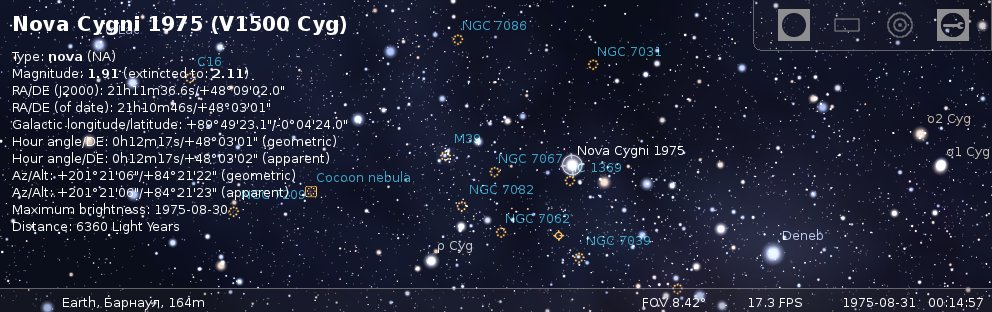
\includegraphics[width=\textwidth]{NovaCygni1975wiki.jpg}
\caption{Nova Cygni 1975 (also known as \textbf{V1500 Cyg})}
\label{fig:NovaCygni1975}
\end{figure}


\noindent The Bright Novae plugin provides visualization of some
bright novae in the Milky Way galaxy.
If enabled (see section~\ref{sec:Plugins:EnablingPlugins}), bright
novae from the past will be presented in the sky at the correct
times. For example, set date and time to 30 August 1975, look at the constellation \emph{Cygnus} to see
\emph{Nova Cygni 1975}\footnote{\url{https://en.wikipedia.org/wiki/V1500_Cygni}} (Fig.~\ref{fig:NovaCygni1975}).


\subsection{Section \big[Novae\big] in config.ini file}
%\label{sec:plugins:BrightNovae:configuration}

You can edit \file{config.ini} file by yourself for changes of the
settings for the Bright Novae plugin -- just make it carefully!

\noindent%
\begin{tabularx}{\textwidth}{l|l|X}\toprule
\emph{ID}            & \emph{Type} & \emph{Description}\\\midrule
last\_update            & string & Date and time of last update\\%\midrule
update\_frequency\_days & int    & Frequency of updates, in days\\%\midrule
updates\_enable         & bool   & Enable updates of bright novae catalog from Internet \\%\midrule
url                     & string & URL of bright novae catalog \\\bottomrule
\end{tabularx}

\subsection{Format of bright novae catalog}
\label{sec:plugins:BrightNovae:format}

To add a new nova, open a new line after line 5 and paste the following, note commas and brackets, they are important:

\begin{configfile}
"Nova designation":
{
    "name": "name of nova",
    "type": "type of nova",
    "maxMagnitude": value of maximal visual magnitude,
    "minMagnitude": value of minimal visual magnitude,
    "peakJD": JD for maximal visual magnitude,
    "m2": Time to decline by 2mag from maximum (in days),
    "m3": Time to decline by 3mag from maximum (in days),
    "m6": Time to decline by 6mag from maximum (in days),
    "m9": Time to decline by 9mag from maximum (in days),
    "distance": value of distance between nova and 
                Earth (in thousands of Light Years),
    "RA": "Right ascension (J2000)",
    "Dec": "Declination (J2000)"
},
\end{configfile}

\noindent For example, the record for \textbf{Nova Cygni 1975} (\textbf{V1500 Cyg}) looks like:
\begin{configfile}
"V1500 Cyg":
{
    "name": "Nova Cygni 1975",
    "type": "NA",
    "maxMagnitude": 1.69,
    "minMagnitude": 21,
    "peakJD": 2442655,
    "m2": 2,
    "m3": 4,
    "m6": 32,
    "m9": 263
    "distance": 6.36,
    "RA": "21h11m36.6s",
    "Dec": "48d09m02s"
},
\end{configfile}

\subsection{Light curves}
\label{sec:plugins:BrightNovae:lightcurves}

This plugin uses a very simple model for calculation of light curves for
novae stars. This model is based on time for decay by $N$
magnitudes from the maximum value, where $N$ is 2, 3, 6 and 9. If a
nova has no values for decay of magnitude then this plugin will use
generalized values for it.

\newpage

\section{Historical Supernovae Plugin}
\label{sec:plugins:HistoricalSupernovae}

\begin{figure}[ht]
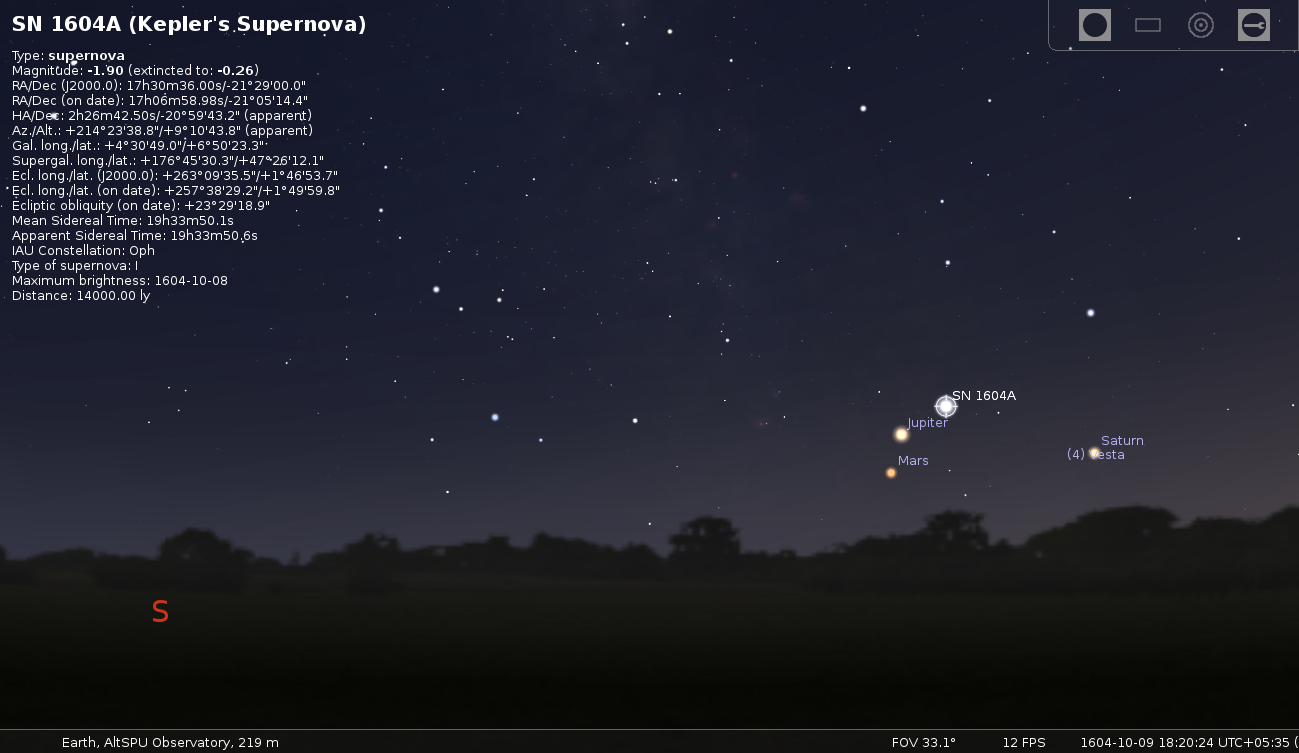
\includegraphics[width=\textwidth]{sn1604wiki.png}
\caption{Supernova 1604 (also known as \textbf{Kepler's Supernova}, \textbf{Kepler's Nova} or \textbf{Kepler's Star})}
\label{fig:SN1604}
\end{figure}


\noindent Similar to the Historical Novae plugin
(section~\ref{sec:plugins:BrightNovae}), the Historical Supernovae
plugin provides visualization of bright historical supernovae
(Fig.~\ref{fig:SN1604}) from the table below.
If enabled (see section~\ref{sec:Plugins:EnablingPlugins}), bright
supernovae from the past will be presented in the sky at the correct
times. For example, set date and time to 29 April 1006, and look at the constellation \emph{Lupus} to see \emph{SN 1006A}.


\subsection{List of supernovae in default catalog}
\label{sec:plugins:HistoricalSupernovae:list}


\begin{longtable}{l|l|l|l|l}\toprule
\emph{Supernova}            & \emph{Date of max. brightness} & \emph{Max. apparent mag.} & \emph{Type} & \emph{Name} \\\midrule
SN 185A\footnote{\url{https://en.wikipedia.org/wiki/SN_185}} & 7 December & -6.0 & Ia & \\\midrule
SN 386A & 24 April & 1.5 & II & \\\midrule
SN 1006A\footnote{\url{https://en.wikipedia.org/wiki/SN_1006}} & 29 April & -7.5 & I & \\\midrule
SN 1054A\footnote{\url{https://en.wikipedia.org/wiki/SN_1054}} & 3 July & -6.0 & II & \\\midrule
SN 1181A\footnote{\url{https://en.wikipedia.org/wiki/SN_1181}} & 4 August & -2.0 & II & \\\midrule
SN 1572A\footnote{\url{https://en.wikipedia.org/wiki/SN_1572}} & 5 November & -4.0 & I & Tycho's Supernova\\\midrule
SN 1604A\footnote{\url{https://en.wikipedia.org/wiki/SN_1604}} & 8 October & -2.0 & I & Kepler's Supernova\\\midrule
SN 1680A\footnote{\url{https://en.wikipedia.org/wiki/Cassiopeia_A}} & 15 August & 6.0 & IIb & Cassiopeia A\\\midrule
SN 1885A\footnote{\url{https://en.wikipedia.org/wiki/S_Andromedae}} & 17 August & 5.8 & IPec & S Andromedae\\\midrule
SN 1895B &  5 July      & 8.0   & I   & \\\midrule
SN 1919A & 14 March     & 11.0  & I   & \\\midrule
SN 1920A & 17 December  & 11.7  & II  & \\%\midrule
SN 1921C & 11 December  & 11.0  & I   & \\\midrule
SN 1937C & 21 August    & 8.5   & Ia  & \\%\midrule
SN 1937D & 15 September & 11.87 & Ia  & \\\midrule
SN 1960F & 21 April     & 11.6  & Ia  & \\%\midrule
SN 1960R & 19 December  & 12.0  & I   & \\%\midrule
SN 1961H &  8 May       & 11.8  & Ia  & \\%\midrule
SN 1962M & 26 November  & 11.5  & II  & \\%\midrule
SN 1965I & 19 Juni      & 11.8  & Ia  & \\%\midrule
SN 1966J &  2 December  & 11.3  & I   & \\%\midrule
SN 1968L & 12 July      & 11.9  & IIP & \\\midrule
SN 1970G & 30 July      & 11.4  & IIL & \\%\midrule
SN 1971I & 29 May       & 11.9  & Ia  & \\%\midrule
SN 1972E\footnote{\url{https://en.wikipedia.org/wiki/SN1972e}} & 8 May & 8.4 & Ia & \\%\midrule
SN 1974G & 27 April     & 11.8  & Ia  & \\%\midrule
SN 1979C & 15 April     & 11.6  & IIL & \\\midrule
SN 1980K & 31 October   & 11.6  & IIL & \\%\midrule
SN 1981B &  9 March     & 12.0  & Ia  & \\%\midrule
SN 1983N & 17 July      & 11.4  & Ib  & \\%\midrule
SN 1986G & 12 May       & 11.44 & Ia Pec & \\%\midrule
SN 1987A\footnote{\url{https://en.wikipedia.org/wiki/SN_1987A}} & 24 February & 2.9 & IIPec & \\%\midrule
SN 1989B &  6 February  & 11.9  & Ia    & \\\midrule
SN 1991T & 26 April     & 11.6  & IaPec & \\%\midrule
SN 1993J\footnote{\url{https://en.wikipedia.org/wiki/SN_1993J}} & 30 March & 10.8 & IIb & \\%\midrule
SN 1994ae & 12 January  & 12.0    & Ia  & \\%\midrule
SN 1994D  & 31 March    & 11.8    & Ia  & \\%\midrule
SN 1998bu & 21 May      & 11.9    & Ia  & \\\midrule
SN 2004dj & 31 July     & 11.3    & IIP & \\%\midrule
SN 2004et &  2 October  & 11.57   & II  & \\\midrule
SN 2011fe\footnote{\url{https://en.wikipedia.org/wiki/SN_2011fe}} & 13 September & 10.06 & Ia & \\%\midrule
SN 2012cg  &  6 Juni     & 11.954 & Ia & \\%\midrule
SN 2012fr  & 16 November & 11.95  & Ia & \\%\midrule
SN 2013aa  & 13 February & 11.9   & Ia & \\%\midrule
SN 2014j   & 30 January  & 10.5   & Ia & \\%\midrule
SN 2017cbv & 22 March    & 11.5   & Ia & \\\bottomrule
\end{longtable}

\subsection{Light curves}
\label{sec:plugins:HistoricalSupernovae:lightcurves}

In this plugin a simple model of light curves for different supernovae
has been implemented (Figure~\ref{fig:SNTypeI+II}). 
%% GZ I try to save 1 page by combining the figures. 
While Type~I supernovae show a peak and slow but steady decay, Type~II supernovae show a longer ``plateau'' in the decay curve.

%A typical light curve used in the plugin for
%supernova type~I is shown in Fig.~\ref{fig:SNTypeI} (bottom scale in
%days).

\begin{figure}[ht]
\begin{center}
%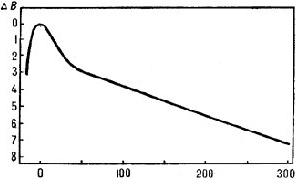
\includegraphics[width=250px]{sn_type_I.jpg}
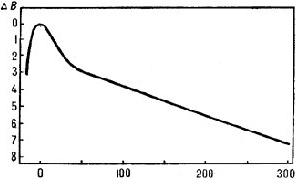
\includegraphics[height=40mm]{sn_type_I.png}\,
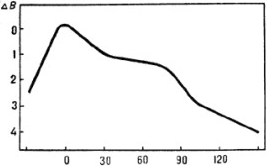
\includegraphics[height=40mm]{sn_type_II.png}
\end{center}
%\caption{Light Curve of Supernova Type I}
%\label{fig:SNTypeI}
\caption{Light Curves of Supernovae Types I (left) and II (right)}
\label{fig:SNTypeI+II}
\end{figure}

%For supernova type~II we use a typical light curve with plateau, which
%you can see in Fig.~\ref{fig:SNTypeII} (bottom scale in days).

%\begin{figure}[ht]
%\begin{center}
%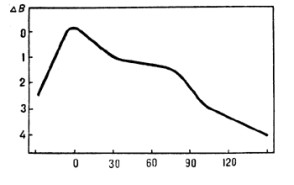
\includegraphics[width=260px]{sn_type_II.jpg}
%\end{center}
%\caption{Light Curve of Supernova Type II}
%\label{fig:SNTypeII}
%\end{figure}

In both images for light curves the maximum brightness is marked as day 0.

\subsection{Section \big[Supernovae\big] in config.ini file}
%\label{sec:plugins:HistoricalSupernovae:configuration}

You can edit \file{config.ini} file by yourself for changes of the
settings for the Historical Supernovae plugin -- just make it carefully!

\noindent%
\begin{tabularx}{\textwidth}{l|l|X}\toprule
\emph{ID}            & \emph{Type} & \emph{Description}\\%\midrule
last\_update            & string & Date and time of last update\\%\midrule
update\_frequency\_days & int    & Frequency of updates, in days\\%\midrule
updates\_enable         & bool   & Enable updates of bright novae catalog from Internet \\%\midrule
url                     & string & URL of bright novae catalog \\\bottomrule
\end{tabularx}

\newpage
\subsection{Format of historical supernovae catalog}
\label{sec:plugins:HistoricalSupernovae:format}

To add a new nova, open a new line after line 5 and paste the following, note commas and brackets, they are important:

\begin{configfile}
"Supernova designation":
{
    "type": "type of supernova",
    "maxMagnitude": value of maximal visual magnitude,
    "peakJD": JD for maximal visual magnitude,
    "alpha": "Right ascension (J2000)",
    "delta": "Declination (J2000)",
    "distance": value of distance between supernova and 
                Earth (in thousands of Light Years),
    "note": "notes for supernova"
},
\end{configfile}

\noindent For example, the record for \textbf{SN 1604A} (\textbf{Kepler's Supernova}) looks like:
\begin{configfile}
"1604A":
{
    "type": "I",
    "maxMagnitude": -2,
    "peakJD": 2307190,
    "alpha": "17h30m36.00s",
    "delta": "-21d29m00.0s",
    "distance": 14,
    "note": "Kepler's Supernova"
},
\end{configfile}

\newpage

\section{Exoplanets Plugin}
\label{sec:plugins:Exoplanets}

\begin{figure}[h]
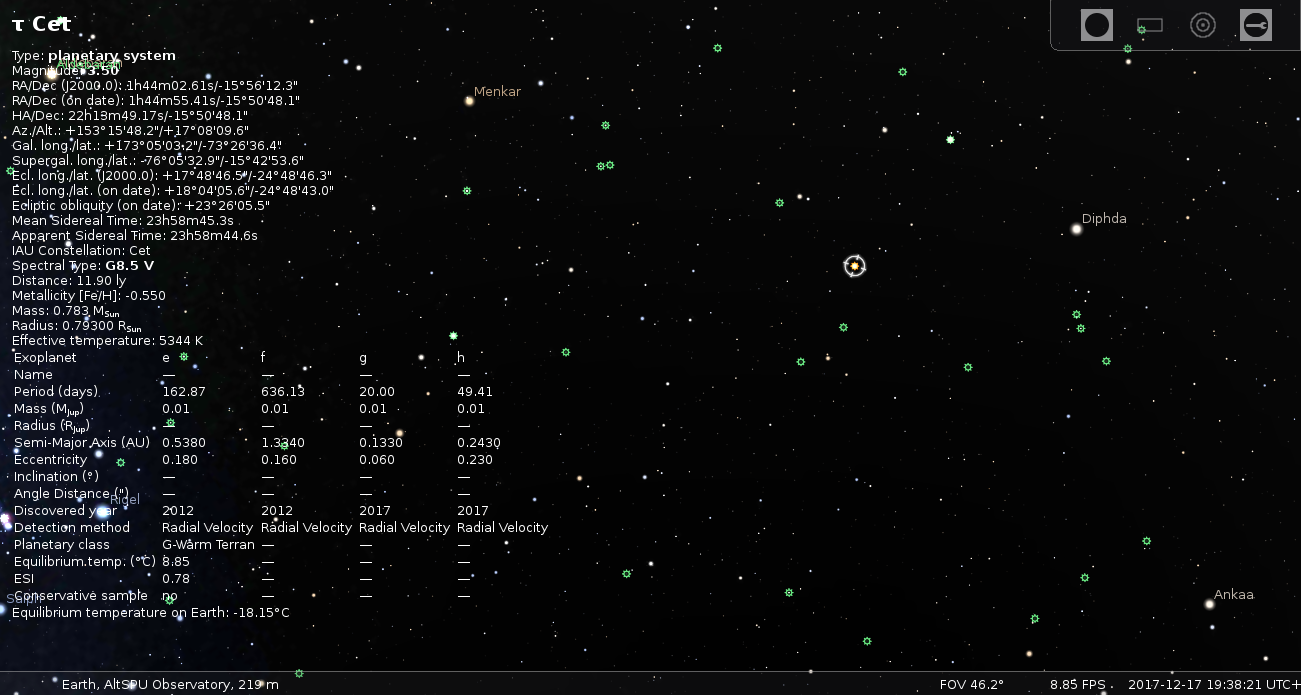
\includegraphics[width=\textwidth]{exoplanets.png}
\caption{Planetary system $\tau$ Ceti}
\label{fig:Exoplanets}
\end{figure}

\noindent This plugin plots the position of stars with
exoplanets. Exoplanets data is derived from ``The Extrasolar Planets
Encyclopaedia''\footnote{\url{http://exoplanet.eu/}}. List of
potential habitable exoplanets and data about them were taken from
``The Habitable Exoplanets
Catalog''\footnote{\url{http://phl.upr.edu/projects/habitable-exoplanets-catalog}}
by the Planetary Habitability
Laboratory\footnote{\url{http://phl.upr.edu/home}}.  If enabled (see
section~\ref{sec:Plugins:EnablingPlugins}), just click on the
Exoplanet button \guibutton{0.6}{btExoplanets-off.png} on the bottom
toolbar to display markers for the stars with known exoplanets. You
can then either click on such a marked star or find the stars with
exoplanets by their designation (e.g., \emph{24 Sex}) in the \key{F3} dialog (see~\ref{sec:gui:search}).


\subsection{Potential habitable exoplanets}
\label{sec:plugins:Exoplanets:habitable}
This plugin can display potential habitable exoplanets (orange marker) and some information about those planets.

\begin{description}
\item[Planetary Class] Planet classification from host star spectral
  type (F, G, K, M; see
  section~\ref{sec:Phenomena:SpectralTypeLuminosityClass}), habitable
  zone (hot, warm, cold) and size (miniterran, subterran, terran,
  superterran, jovian, neptunian) (Earth = G-Warm Terran).
\item[Equilibrium Temperature] The planetary equilibrium
  temperature\footnote{\url{https://en.wikipedia.org/wiki/Planetary_equilibrium_temperature}}
  is a theoretical temperature (in \degree C) that the planet would be
  at when considered simply as if it were a black body being heated
  only by its parent star (assuming a 0.3 bond albedo). As example the
  planetary equilibrium temperature of Earth is -18.15\degree C (255~K).
\item[Earth Similarity Index (ESI)] Similarity to
  Earth\footnote{\url{http://phl.upr.edu/projects/earth-similarity-index-esi}}
  on a scale from 0 to 1, with 1 being the most Earth-like. ESI
  depends on the planet's radius, density, escape velocity, and
  surface temperature.
\end{description}

\subsection{Proper names}
\label{sec:plugins:Exoplanets:ProperNames}
In December 2015\footnote{%
  \url{https://www.iau.org/news/pressreleases/detail/iau1514/}} and in December 2019\footnote{%
      \url{https://www.iau.org/news/pressreleases/detail/iau1912/}}, the International Astronomical Union (IAU)\index{IAU} has officially approved names for several exoplanets after a public vote.
\begin{description}
\item[Veritate]* (14 And) -- From the latin Veritas, truth. The ablative form means \textit{where there is truth}\footnote{The original name proposed, Veritas, is that of an asteroid important for the study of the solar system.}.
\item[Spe]* (14 And b) -- From the latin Spes, hope. The ablative form means \textit{where there is hope}.
\item[Musica] (18 Del) -- Musica is Latin for \textit{music}.
\item[Arion] (18 Del b) -- Arion was a genius of poetry and music in ancient Greece. According to legend, his life was saved at sea by dolphins after attracting their attention by the playing of his kithara.
\item[Fafnir] (42 Dra) -- Fafnir was a Norse mythological dwarf who turned into a dragon.
\item[Orbitar] (42 Dra b) -- Orbitar is a contrived word paying homage to the space launch and orbital operations of NASA.
\item[Chalawan] (47 UMa) -- Chalawan is a mythological crocodile king from a Thai folktale.
\item[Taphao Thong] (47 UMa b) -- Taphao Thong is one of two sisters associated with the Thai folk tale of Chalawan.
\item[Taphao Kaew] (47 UMa c) -- Taphao Kae is one of two sisters associated with the Thai folk tale of Chalawan.
\item[Helvetios] (51 Peg) -- Helvetios is Celtic for the \textit{Helvetian} and refers to the Celtic tribe that lived in Switzerland during antiquity.
\item[Dimidium] (51 Peg b) -- Dimidium is Latin for \textit{half}, referring to the planet's mass of at least half the mass of Jupiter.
\item[Copernicus] (55 Cnc) -- Nicolaus Copernicus or Mikolaj Kopernik (1473-1543) was a Polish astronomer who proposed the heliocentric model of the solar system in his book ``De revolutionibus orbium coelestium''.
\item[Galileo] (55 Cnc b) -- Galileo Galilei (1564-1642) was an Italian astronomer and physicist often called the \textit{father of observational astronomy} and the \textit{father of modern physics}. Using a telescope, he discovered the four largest satellites of Jupiter, and the reported the first telescopic observations of the phases of Venus, among other discoveries.
\item[Brahe] (55 Cnc c) -- Tycho Brahe (1546-1601) was a Danish astronomer and nobleman who recorded accurate astronomical observations of the stars and planets. These observations were critical to Kepler's formulation of his three laws of planetary motion.
\item[Lipperhey]* (55 Cnc d) -- Hans Lipperhey (1570-1619) was a German-Dutch lens grinder and spectacle maker who is often attributed with the invention of the refracting telescope in 1608\footnote{The original spelling of Lippershey was corrected to Lipperhey on 15.01.2016. The commonly seen spelling Lippershey (with an s) results in fact from a typographical error dating back from 1831, thus should be avoided.}.
\item[Janssen] (55 Cnc e) -- Zacharias Janssen (1580s-1630s) was a Dutch spectacle maker who is often attributed with invention of the microscope, and more controversially with the invention of the telescope.
\item[Harriot] (55 Cnc f) -- Thomas Harriot (ca. 1560-1621) was an English astronomer, mathematician, ethnographer, and translator, who is attributed with the first drawing of the Moon through telescopic observations.
\item[Amateru]* ($\epsilon$ Tau b) -- \textit{Amateru} is a common Japanese appellation for shrines when they enshrine Amaterasu, the Shinto goddess of the Sun, born from the left eye of the god Izanagi\footnote{The name originally proposed, Amaterasu, is already used for an asteroid.}.
\item[Hypatia] ($\iota$ Dra b) -- Hypatia was a famous Greek astronomer, mathematician, and philosopher. She was head of the Neo-Platonic school at Alexandria in the early $5^{th}$ century, until murdered by a Christian mob in 415.
\item[Ran]* ($\epsilon$ Eri) -- Ran is the Norse goddess of the sea, who stirs up the waves and captures sailors with her net.
\item[AEgir]* ($\epsilon$ Eri b) -- {\AE}gir is Ran's husband, the personified god of the ocean. \textit{{\AE}gir} and \textit{Ran} both represent the \textit{Jotuns} who reign in the outer Universe; together they had nine daughters\footnote{Note the typographical difference between {\AE}gir and Aegir, the Norwegian transliteration. The same name, with the spelling Aegir, has been attributed to one of Saturn's satellites, discovered in 2004.}.
\item[Tadmor]* ($\gamma$ Cep b) -- Ancient Semitic name and modern Arabic name for the city of Palmyra, a UNESCO World Heritage Site.
\item[Dagon] ($\alpha$ PsA b) -- Dagon was a Semitic deity, often represented as half-man, half-fish.
\item[Tonatiuh] (HD 104985) -- Tonatiuh was the Aztec god of the Sun.
\item[Meztli] (HD 104985 b) -- Meztli was the Aztec goddess of the Moon.
\item[Ogma]* (HD 149026) -- Ogma was a deity of eloquence, writing, and great physical strength in the Celtic mythologies of Ireland and Scotland, and may be related to the Gallo-Roman deity \textit{Ogmios}\footnote{Ogmios is a name already attributed to an asteroid.}.
\item[Smertrios] (HD 149026 b) -- Smertrios was a Gallic deity of war.
\item[Intercrus] (HD 81688) -- Intercrus means \textit{between the legs} in Latin style, referring to the star's position in the constellation Ursa Major.
\item[Arkas] (HD 81688 b) -- Arkas was the son of Callisto (Ursa Major) in Greek mythology.
\item[Cervantes] ($\mu$ Ara) -- Miguel de Cervantes Saavedra (1547-1616) was a famous Spanish writer and author of ``El Ingenioso Hidalgo Don Quixote de la Mancha''.
\item[Quijote] ($\mu$ Ara b) -- Lead fictional character from Cervantes's ``El Ingenioso Hidalgo Don Quixote de la Mancha''.
\item[Dulcinea]($\mu$ Ara c) — Fictional character and love interest of Don Quijote (or Quixote) in Cervantes's ``El Ingenioso Hidalgo Don Quixote de la Mancha''.
\item[Rocinante] ($\mu$ Ara d) -- Fictional horse of Don Quijote in Cervantes's ``El Ingenioso Hidalgo Don Quixote de la Mancha''.
\item[Sancho] ($\mu$ Ara e) -- Fictional squire of Don Quijote in Cervantes's ``El Ingenioso Hidalgo Don Quixote de la Mancha''.
\item[Thestias]* ($\beta$ Gem b) -- Thestias is the patronym of Leda and her sister Althaea, the daughters of Thestius. Leda was a Greek queen, mother of Pollux and of his twin Castor, and of Helen and Clytemnestra\footnote{The original proposed name Leda is already attributed to an asteroid and to one of Jupiter's satellites. The name Althaea is also attributed to an asteroid.}.
\item[Lich] (PSR B1257+12) -- Lich is a fictional undead creature known for controlling other undead creatures with magic.
\item[Draugr] (PSR B1257+12 b) -- Draugr refers to undead creatures in Norse mythology.
\item[Poltergeist] (PSR B1257+12 c) -- Poltergeist is a name for supernatural beings that create physical disturbances, from German for noisy ghost.
\item[Phobetor] (PSR B1257+12 d) -- Phobetor is a Greek mythological deity of nightmares, the son of Nyx, the primordial deity of night.
\item[Titawin] ($\upsilon$ And) -- Titawin (also known as Medina of Tetouan) is a settlement in northern Morocco and UNESCO World Heritage Site. Historically it was an important point of contact between two civilizations (Spanish and Arab) and two continents (Europe and Africa) after the $8^{th}$ century.
\item[Saffar] ($\upsilon$ And b) -- Saffar is named for Abu al-Qasim Ahmed Ibn-Abd Allah Ibn-Omar al Ghafiqi Ibn-al-Saffar, who taught arithmetic, geometry, and astronomy in $11^{th}$ century Cordova in Andalusia (modern Spain), and wrote an influential treatise on the uses of the astrolabe.
\item[Samh] ($\upsilon$ And c) -- Samh is named for Abu al-Qasim 'Asbagh ibn Muhammad ibn al-Samh al-Mahri (or Ibn al-Samh), a noted $11^{th}$ century astronomer and mathematician in the school of al Majriti in Cordova (Andalusia, now modern Spain).
\item[Majriti] ($\upsilon$ And d) -- Majriti is named for Abu al-Qasim al-Qurtubi al-Majriti, a notable mathematician, astronomer, scholar, and teacher in $10^{th}$ century and early $11^{th}$ century Andalusia (modern Spain).
\item[Libertas]* ($\xi$ Aql) -- Libertas is Latin for liberty. Liberty refers to social and political freedoms, and a reminder that there are people deprived of liberty in the world even today. The constellation Aquila represents an eagle -- a popular symbol of liberty.
\item[Fortitudo]* ($\xi$ Aql b) -- Fortitudo is Latin for fortitude. Fortitude means emotional and mental strength in the face of adversity, as embodied by the eagle (represented by the constellation Aquila).
% IAU:iau1912
\item[Illyrian] (HD 82886) -- Historians largely believe that the Albanians are descendants of the Illyrians, a term Albanians proudly call themselves.
\item[Arber] (HD 82886 b) -- Arber is the term for the inhabitants of Albania during the middle ages.
\item[Hoggar] (HD 28678) -- Hoggar is the name of the main mountain range in the Sahara Desert in southern Algeria.
\item[Tassili] (HD 28678 b) -- Tassili is a UNESCO World Heritage Site situated in the Sahara Desert and is renowned for its prehistoric cave art and scenic geological formations.
\item[Arcalís] (HD 131496) -- Arcalis is a famous peak in the north of Andorra, where the Sun passes through a hole in the mountain twice a year at fixed dates. It was used as a primitive solar calendar and reference point for shepherds and early inhabitants of Andorra.
\item[Madriu] (HD 131496 b) -- Madriu (\textit{Mare del riu} in Catalan, \textit{Mother of the River} in English) is the name of a glacial valley and of the river that runs through it in the southeast of Andorra. It is the main part of the Madriu-Perafita-Claror UNESCO World Heritage Site.
\item[Nosaxa] (HD 48265) -- Nosaxa means \textit{spring} in the Moqoit language. The word comes from a combination of nosahuec, which means renew, and ñaaxa, which means \textit{year}.
\item[Naqaya] (HD 48265 b) -- Naqaya means \textit{brother-family-relative} in the Moqoit language and leads us to call all humans, indigenous or non-indigenous, brother.
\item[Malmok] (WASP-39) -- Malmok is an indigenous name given to a beach in Aruba with a narrow sandy stretch that interrupts the limestone and rocky terrace along the coast. Its shallow clear Caribbean waters make it a popular snorkelling spot.
\item[Bocaprins] (WASP-39 b) -- Boca Prins is a secluded beach with white dunes and iconic scenery situated in Arikok National Park along the northeast coast of Aruba. It is named after Plantation Prins where coconuts are cultivated.
\item[Bubup] (HD 38283) -- Bubup is the Boonwurrung word for child.
\item[Yanyan] (HD 38283 b) -- YanYan is the Boonwurrung word for boy.
\item[Franz] (HAT-P-14) -- Franz is a character in the movie ``Sissi'' embodying an emperor of Austria in the $19^{th}$ century. The role is played by the actor Karlheinz Böhm.
\item[Sissi] (HAT-P-14 b) -- Sissi is a character in the movie ``Sissi'', who is married with Franz. The role is played by the actress Romy Schneider.
\item[Mahsati] (HD 152581) -- Mahsati Ganjavi (1089--1159) is one of the brightest shining stars of Azerbaijani poetry. She was said to have associated with both Omar Khayyam and Nizami and was well educated and talented and played numerous musical instruments.
\item[Ganja] (HD 152581 b) -- Ganja is an ancient city of Azerbaijan, and is the birth place of many prominent people such as the poets Mahsati and Nizami. It is the ancient capital of Azerbaijan, the first capital of the Azerbaijan Democratic Republic and the city with the spirit of wisdom and freedom.
\item[Timir] (HD 148427) -- Timir means darkness in Bengali language, alluding to the star being far away in the darkness of space.
\item[Tondra] (HD 148427 b) -- Tondra means \textit{nap} in Bengali language, alluding to the symbolic notion that the planet was asleep until discovered.
\item[Nervia] (HD 49674) -- Nervia, adapted from Nervii, was a prominent Belgian Celtic tribe.
\item[Eburonia] (HD 49674 b) -- Eburonia, adapted from Eburones, was a prominent Belgian Celtic tribe.
\item[Gakyid] (HD 73534) -- Gakyid means \textit{happiness}. Gross National Happiness is the development philosophy conceived and followed in Bhutan and is one of Bhutan's contributions to the world.
\item[Drukyul] (HD 73534 b) -- Drukyul (land of the thunder dragon) is the native name for Bhutan, the country that came up with the philosophy of Gross National Happiness.
\item[Tapecue] (HD 63765) -- Tapecue means \textit{eternal path} in Guarani and represents the Milky Way through which the first inhabitants of the Earth arrived and could return.
\item[Yvaga] (HD 63765 b) -- Yvaga means \textit{paradise} for the Guarani and the Milky Way was known as the road to Yvaga or paradise.
\item[Bosona] (HD 206610) -- Bosona is the name given to the territory of Bosnia in the $10^{th}$ century. Later, the name was transformed to Bosnia originating from the name of the Bosna river.
\item[Naron] (HD 206610 b) -- Naron is one of the names given to the Neretva river in Herzegovina (and partly in Croatia) in antiquity orginating with the Celts who called it Nera Etwa which means the Flowing Divinity.
\item[Tupi] (HD 23079) -- Tupi is the name of the most populous Indigenous People living on the eastern coast of South America, before the Portuguese arrived in the $16^{th}$ century.
\item[Guarani] (HD 23079 b) -- Guarani is the name of the most populous Indigenous people living in South Brazil and parts of Argentina, Paraguay and Uruguay.
\item[Gumala] (HD 179949) -- Gumala is a Malay word, which means a magic bezoar stone found in snakes, dragons, etc.
\item[Mastika] (HD 179949 b) -- Mastika is a Malay word, which means \textit{a gem, precious stone, jewel} or \textit{the prettiest, the most beautiful}.
\item[Tangra] (WASP-21) -- Tangra is the supreme celestial god that early Bulgars worshiped.
\item[Bendida] (WASP-21 b) -- Bendida is the Great Mother Goddess of the Thracians. She was especially revered as a goddess of marriage and living nature.
\item[Mouhoun] (HD 30856) -- Mouhoun, also called Volta Noire, is the largest river in Burkina Faso and plays an important role in the lives of the people in the areas it passes through.
\item[Nakanbé] (HD 30856 b) -- The Nakanbé, also called Volta Blanche, is the second largest river in Burkina Faso. Its source is in the heart of the Sahara Burkinabe and ends in Ghana.
\item[Nikawiy] (HD 136418) -- Nikawiy is the word for mother in the Indigenous Cree language of Canada.
\item[Awasis] (HD 136418 b) -- Awasis is the word for child in the Indigenous Cree language of Canada.
\item[Pincoya] (HD 164604) -- Pincoya is a female water spirit from southern Chilean mythology who is said to bring drowned sailors to the Caleuche so that they can live in the afterlife.
\item[Caleuche] (HD 164604 b) -- Caleuche is a large ghost ship from southern Chilean mythology which sails the seas around the island of Chiloé at night.
\item[Lionrock] (HD 212771) -- Lion Rock is a lion-shaped peak overlooking Hong Kong and is a cultural symbol with deep respect from the local community.
\item[Victoriapeak] (HD 212771 b) -- Victoria Peak overlooks the bustling Victoria Harbour and is regarded as an ambassadorial gateway for foreign visitors wishing to experience Hong Kong first hand.
\item[Xihe] (HD 173416) -- Xiheis the goddess of the sun in the Chinese mythology and also represents the earliest astronomers and developers of calendars in ancient China.
\item[Wangshu] (HD 173416 b) -- Wangshu is the goddess who drives for the Moon and also represents the Moon in Chinese mythology.
\item[Formosa] (HD 100655) -- Formosa is the historical name of Taiwan used in the $17^{th}$ century, meaning beautiful in Latin.
\item[Sazum] (HD 100655 b) -- Sazum is the traditional name of Yuchi, a Township in Nantou county, in which the famous Sun-Moon Lake lies. Sazum means water in the language of the Thao people who are a tribe of Taiwanese aborigines who lived in the region for hundreds of years.
\item[Macondo] (HD 93083) -- Macondo is the mythical village of the novel ``One Hundred Years of Solitude'' (``Cien años de soledad'') the classic novel by Gabriel García Marquez. Macondo is a fictional place where magic and reality are mixed.
\item[Melquíades] (HD 93083 b) -- Melquíades is a fictional character that walks around Macondo, like a planet orbiting a star, connecting it with the external world by introducing new knowledge using his inventions as well as his stories.
\item[Poerava] (HD 221287) -- Poerava is the word in the Cook Islands Maori language for a large mystical black pearl of utter beauty and perfection.
\item[Pipitea] (HD 221287 b) -- Pipitea is a small, white and gold pearl found in Penrhyn lagoon in the northern group of the Cook Islands.
\item[Dìwö] (WASP-17) -- Dìwö in Bribri language means \textit{the sun (bigger than the sun we know)} and that never turns off.
\item[Ditsö] (WASP-17 b) -- Ditsö is the name that the god Sibö gave to the first Bribri people.
\item[Stribor] (HD 75898) -- Stribor is God of winds in Slavic mythology, as well as a literature character in the book Priče iz davnine (Croatian Tales of Long Ago) by the Croatian author Ivana Brlić-Mažuranić.
\item[Veles] (HD 75898 b) -- Veles is a major Slavic god of earth, waters and the underworld.
\item[Felixvarela] (BD-17 63) -- Felix Varela (1788–1853) was the first to teach science in Cuba at the San Carlos and San Ambrosio Seminary. He opened the way to education for all, and began the experimental teaching of physics in Cuba.
\item[Finlay] (BD-17 63 b) -- Carlos Juan Finlay (1833–1915) was an epidemiologist recognized as a pioneer in the research of yellow fever, determining that it was transmitted through mosquitoes.
\item[Alasia] (HD 168746) -- Alasia is the first historically recorded name of Cyprus, dating back to mid-fifteenth century BC.
\item[Onasilos] (HD 168746 b) -- Onasilos is the oldest historically recorded doctor in Cyprus, inscribed on the fifth century BC Idalion Tablet. Also known as the Onasilou Plate, it is considered as the oldest legal contract found in the world.
\item[Absolutno] (XO-5) -- Absolutno is a fictional miraculous substance in the sci-fi novel ``Továrna na absolutno'' (``The Factory for the Absolute'') by influential Czech writer Karel {\v{C}}apek.
\item[Makropulos] (XO-5 b) -- Makropulos is the name from Karel {\v{C}}apek's play Věc Makropulos (The Makropulos Affair), dealing with problems of immortality and consequences of an artificial prolongation of life.
\item[Muspelheim] (HAT-P-29) -- Muspelheim is the Norse mythological realm of fire. The first gods used the sparks of Muspelheim to form the sun, moon, planets, and stars.
\item[Surt] (HAT-P-29 b) -- Surt is the ruler of Muspelheim and the fire giants there in Norse mythology. At Ragnarok, the end of the world, he will lead the attack on our world and destroy it in flames.
\item[Márohu] (WASP-6) -- Márohu the god of drought is the protector of the Sun and is engraved at a higher position on the stalagmite than Boinayel in the El Puente cave, where the Sun makes its way down every 21 December.
\item[Boinayel] (WASP-6 b) -- Boinayel the god of rain that fertilizes the soil is engraved on the stalagmite at a lower position than Márohu in the El Puente cave.
\item[Nenque] (HD 6434) -- Nenque means \textit{the Sun} in the language spoken by the Indigenous Waorani tribes of the Amazon regions of Ecuador
\item[Eyeke] (HD 6434 b) -- Eyeke means \textit{near} in the language spoken by the Indigenous Waorani tribes of the Amazon regions of Ecuador. This word is suggested for the exoplanet owing to the proximity of the planet to the host star.
\item[Citalá] (HD 52265) -- Citalá means \textit{River of stars} in the native Nahuat language.
\item[Cayahuanca] (HD 52265 b) -- Cayahuanca means \textit{The rock looking at the stars} in the native Nahuat language.
\item[Koit] (XO-4) -- Koit is Estonian for the time when the Sun rises in the morning (dawn).
\item[Hämarik] (XO-4 b) -- Hämarik is Estonian for the time when the Sun goes down in the evening (twilight).
\item[Buna] (HD 16175) -- Buna is the commonly used word for coffee in Ethiopia.
\item[Abol] (HD 16175 b) -- Abol is the first of three rounds of coffee in the Ethiopian traditional coffee ceremony.
\item[Horna] (HAT-P-38) -- Horna is hell or the underworld from Finnic mythology.
\item[Hiisi] (HAT-P-38 b) -- Hiisi represents sacred localities and later evil spirits from Finnic mythology.
\item[Bélénos] (HD 8574) -- Bélénos was the god of light, of the Sun, and of health in Gaulish mythology.
\item[Bélisama] (HD 8574 b) -- Bélisama was the goddess of fire, notably of the hearth and of metallurgy and glasswork, in Gaulish mythology.
\item[Itonda] (HD 208487) -- Itonda, in the Myene tongue, corresponds to all that is beautiful.
\item[Mintome] (HD 208487 b) -- Mintome, in the Fang tongue, is a mythical land where a brotherhood of brave men live.
\item[Mago] (HD 32518) -- Mago is a National Park in Ethiopia noted for its giraffes. The star also happens to be in the constellation of Camelopardis (the giraffe).
\item[Neri] (HD 32518 b) -- The Neri river in Ethiopia runs through parts of the Mago National park.
\item[Sika] (HD 181720) -- Sika means \textit{gold} in the Ewe language and gold is one of Ghana's principal exports.
\item[Toge] (HD 181720 b) -- Toge means \textit{earring} in the Ewe language.
\item[Lerna] (HAT-P-42) -- Lerna was the name of a lake in the eastern Peloponnese, where the Lernaean Hydra, an immortal mythical nine-headed beast lived. The star lies in the constellation of Hydra.
\item[Iolaus] (HAT-P-42 b) -- Iolaus was the nephew of Heracles from Greek mythology, moving around lake Lerna in helping Heracles to exterminate the Lernaean Hydra. Similarly this exoplanet in the constellation of Hydra moves around its parent star.
\item[Tojil] (WASP-22) -- Tojil is the name of one of the Mayan deities related to rain, storms, and fire.
\item[Koyopa'] (WASP-22 b) -- Koyopa' is the word associated with lightning in K'iche' (Quiché) Mayan language.
\item[Citadelle] (HD 1502) -- The Citadelle is a large mountaintop fortress in Nord, Haiti built after Haiti's independence, and was designated a UNESCO World Heritage site along with the nearby Sans-Souci Palace.
\item[Indépendance] (HD 1502 b) -- Indépendance is named after the Haitian Declaration of Independence on 1 January 1804, when Haiti became the first independent black republic.
\item[Hunahpú] (HD 98219) -- Hunahpú was one of the twin gods who became the Sun in K'iche' (Quiché) Mayan mythology as recounted in the Popol Vuh.
\item[Ixbalanqué] (HD 98219 b) -- Ixbalanqué was one of the twin gods who became the Moon in K'iche' (Quiché) Mayan mythology as recounted in the Popol Vuh.
\item[Hunor] (HAT-P-2) -- Hunor was a legendary ancestor of the Huns and the Hungarian nation, and brother of Magor.
\item[Magor] (HAT-P-2 b) -- Magor was a legendary ancestor of the Magyar people and the Hungarian nation, and brother of Hunor.
\item[Funi] (HD 109246) -- Funi is an old Icelandic word meaning \textit{fire} or \textit{blaze}.
\item[Fold] (HD 109246 b) -- Fold is an old Icelandic word meaning \textit{earth} or \textit{soil}.
\item[Bibhā] (HD 86081) -- Bibhā is the Bengali pronunciation of the Sanskrit word Vibha, which means \textit{a bright beam of light}.
\item[Santamasa] (HD 86081 b) -- Santamasa in Sanskrit means \textit{clouded}, which alludes to the exoplanet’s atmosphere.
\item[Dofida] (HD 117618) -- Dofida means \textit{our star} in Nias language.
\item[Noifasui] (HD 117618 b) -- Noifasui means \textit{revolve around} in Nias language, derived from the word ifasui, meaning \textit{to revolve around}, and no, indicating that the action occurred in the past and continued to the present time.
\item[Kaveh] (HD 175541) -- Kaveh is one of the heroes of Shahnameh, the epic poem composed by Persian poet Ferdowsi between 977 and 1010 CE. Kaveh is a blacksmith who symbolises justice.
\item[Kavian] (HD 175541 b) -- Kaveh carries a banner called Derafsh Kaviani (Derafsh: banner, Kaviani: relating to Kaveh).
\item[Uruk] (HD 231701) -- Uruk was an ancient city of the Sumer and Babylonian civilizations in Mesopotamia situated along an ancient channel of the Euphrates river in modern-day Iraq.
\item[Babylonia] (HD 231701 b) -- Babylonia was a key kingdom in ancient Mesopotamia from the $18^{th}$ to $6^{th}$ centuries BC whose name-giving capital city was built on the Euphrates river.
\item[Tuiren] (HAT-P-36) -- Tuiren was the aunt of the hunterwarrior Fionn mac Cumhaill of Irish legend, who was turned into a hound by the jealous fairy Uchtdealbh.
\item[Bran] (HAT-P-36 b) -- Tuiren's son Bran was a hound and cousin of the hunterwarrior Fionn mac Cumhaill of Irish legend.
\item[Tevel] (HAT-P-9) -- Tevel means \textit{Universe} or \textit{everything} and begins with the letter Taf, the last letter in the Hebrew alphabet.
\item[Alef] (HAT-P-9 b) -- Alef is the first letter in the Hebrew alphabet and also means bull.
\item[Flegetonte] (HD 102195) -- Flegetonte is the underworld river of fire from Greek Mythology in the Italian narrative poem on the afterlife ``Divina Commedia'' (``Divine Commedy'') by Dante Alighieri, chosen as an allusion to the star's fiery nature.
\item[Lete] (HD 102195 b) -- Lete is the oblivion river made of fog from Greek Mythology in the Italian narrative poem on the afterlife ``Divina Commedia'' (``Divine Commedy'') by Dante Alighieri, chosen as an allusion to the planet's gaseous nature.
\item[Nyamien] (WASP-15) -- Nyamien refers to the supreme creator deity of Akan mythology.
\item[Asye] (WASP-15 b) -- Asye refers to the Earth goddess of Akan mythology.
\item[Kamui] (HD 145457) -- Kamui is a word in the Ainu language denoting a supernatural entity possessing spiritual energy.
\item[Chura] (HD 145457 b) -- Chura is a word in the Ryukyuan/Okinawan language meaning \textit{natural beauty}.
\item[Petra] (WASP-80) -- Petra is a historical and archaeological city in southern Jordan and a UNESCO World Heritage site.
\item[Wadirum] (WASP-80 b) -- Wadi Rum (Valley of the Moon) is located at the far south of Jordan, it is the largest valley in Jordan, set on the high plateau at the western edge of the Arabian Desert.
\item[Kalausi] (HD 83443) -- The word Kalausi means \textit{a very strong whirling column of wind} in the Dholuo language of Kenya.
\item[Buru] (HD 83443 b) -- Buru means \textit{dust} in the Dholuo language of Kenya and is typically associated with wind storms.
\item[Liesma] (HD 118203) -- Liesma means \textit{flame}, and it is the name of a character from the Latvian poem Staburags un Liesma.
\item[Staburags] (HD 118203 b) -- Staburags is the name of a character from the Latvian poem Staburags un Liesma, and denotes a rock with symbolic meaning in literature and history.
\item[Phoenicia] (HD 192263) -- Phoenicia was an ancient thalassocratic civilisation of the Mediterranean that originated from the area of modern-day Lebanon.
\item[Beirut] (HD 192263 b) -- Beirut is one of the oldest continuously inhabited cities in the world and was a Phoenician port. Beirut is now the capital and largest city of Lebanon.
\item[Pipoltr] (TrES-3) -- In the local dialect of Triesenberg, Pipoltr is a bright and visible butterfly, alluding to the properties of a star.
\item[Umbäässa] (TrES-3 b) -- In the local dialect of southern Liechtenstein, Umbäässa is a small and barely visible ant, alluding to the properties of a planet with respect to its star.
\item[Taika] (HAT-P-40) -- Taika means \textit{peace} in the Lithuanian language.
\item[Vytis] (HAT-P-40 b) -- Vytis is the symbol of the Lithuanian coat of arms.
\item[Lucilinburhuc] (HD 45350) -- The Lucilinburhuc fortress was built in 963 by the founder of Luxembourg, Count Siegfried.
\item[Peitruss] (HD 45350 b) -- Peitruss is derived from the name of the Luxembourg river Pétrusse, with the river's bend around Lucilinburhuc fortress alluding to the orbit of the planet around its star.
\item[Rapeto] (HD 153950) -- Rapeto is a giant creature from Malagasy tales.
\item[Trimobe] (HD 153950 b) -- Trimobe is a rich ogre from Malagasy tales.
\item[Intan] (HD 20868) -- Intan means \textit{diamond} in the Malay language (Bahasa Melayu), alluding to the shining of a star.
\item[Baiduri] (HD 20868 b) -- Baiduri means \textit{opal} in Malay language (Bahasa Melayu), alluding to the mysterious beauty of the planet.
\item[Sansuna] (HAT-P-34) -- Sansuna is the name of the mythological giant from traditional Maltese folk tales that carried the stones of the Gozo megalithic temples on her head.
\item[Ġgantija] (HAT-P-34 b) -- Ġgantija means \textit{giantess}: the megalithic temple complex on the island of Gozo, which alludes to the grandeur of this gas giant exoplanet.
\item[Diya] (WASP-72) -- Diya is an oil lamp that is brought by Indian ancestors to Mauritius in the 1820's, and is used for lighting during special occasions, including the light festival of Diwali.
\item[Cuptor] (WASP-72 b) -- Cuptor is a thermally insulated chamber used for baking or drying substances, that has long disappeared in Mauritius and has been replaced by more sophisticated ovens.
\item[Axólotl] (HD 224693) -- Axólotl means \textit{water animal} in the native Nahuatl language, which is a unique and culturally significant endemic amphibious species from the basin of Mexico.
\item[Xólotl] (HD 224693 b) -- Xólotl means \textit{animal} in the native Nahuatl language and was an Aztec deity associated with the evening star (Venus).
\item[Tislit] (WASP-161) -- Tislit is the name of a lake in the Atlas mountains of Morocco. It means \textit{the bride} in the Amazigh language and it is associated with a heartbroken beautiful girl in an ancient local legend.
\item[Isli] (WASP-161 b) -- Isli is the name of a lake in the Atlas mountains of Morocco. It means \textit{the groom} in the Amazigh language and it is associated with a heartbroken handsome boy in an ancient local legend.
\item[Emiw] (HD 7199) -- Emiw represents love in the local Makhuwa language of the northern region of Mozambique.
\item[Hairu] (HD 7199 b) -- Hairu represents unity in the local Makhuwa language of the northern region of Mozambique.
\item[Ayeyarwady] (HD 18742) -- Ayeyarwady is the largest and most important river in Myanmar.
\item[Bagan] (HD 18742 b) -- Bagan is one of Myanmar's ancient cities that lies beside the Ayeyarwardy river.
\item[Sagarmatha] (HD 100777) -- Sagarmatha is the Nepali name for the highest peak in the world (also known as Mount Everest) and symbol of national pride of Nepal.
\item[Laligurans] (HD 100777 b) -- Laligurans are the Nepali variation of the rhododendron flower and is the national flower of Nepal.
\item[Sterrennacht] (HAT-P-6) -- The Sterrennacht (Starry Night) is a world-famous painting by Dutch grand master Van Gogh that was painted in France in 1889 and now belongs to the permanent collection of New York's Museum of Modern Art.
\item[Nachtwacht] (HAT-P-6 b) -- The Nachtwacht (Night Watch) is a world-famous painting by Dutch grand master Rembrandt that was completed in 1642 and now belongs to the collection of the Rijksmuseum in Amsterdam.
\item[Karaka] (HD 137388) -- Karaka is the word in the Māori language for a plant endemic to New Zealand that produces a bright orange, fleshy fruit.
\item[Kererū] (HD 137388 b) -- Kererū is the word in the Māori language for a large bush pigeon native to New Zealand.
\item[Cocibolca] (HD 4208) -- Cocibolca is the Nahualt name for the largest lake in Central America in Nicaragua.
\item[Xolotlan] (HD 4208 b) -- Xolotlan is the name of the second largest lake of Nicaragua and its name is from the Nahualt language of the indigenous tribe that settled in Nicaragua, which symbolises a native god and a refuge for animals.
\item[Amadioha] (HD 43197) -- Amadioha is the god of thunder in Igbo mythology. As well as representing justice, Amadioha is also a god of love, peace and unity.
\item[Equiano] (HD 43197 b) -- Equiano was a writer and abolitionist from Ihiala, Nigeria who fought injustice and the elimination of the slave trade.
\item[Násti] (HD 68988) -- Násti means \textit{star} in the Northern Sami language of Norway.
\item[Albmi] (HD 68988 b) -- Albmi means \textit{sky} in the Northern Sami language of Norway.
\item[Shama] (HAT-P-23) -- Shama is an Urdu literary term meaning \textit{a small lamp} or \textit{flame}, symbolic of the light of the star.
\item[Perwana] (HAT-P-23 b) -- Perwana means \textit{moth} in Urdu, alluding to the eternal love of an object circling the source of light (the lamp).
\item[Moriah] (HD 99109) -- Moriah is an ancient name for the mountain within the Old City of Jerusalem.
\item[Jebus] (HD 99109 b) -- Jebus was the ancient name of Jerusalem in $2^{nd}$ millennium BC when populated by the Canaanite tribe of Jebusites.
\item[Montuno] (WASP-79) -- Montuno is the traditional costume the man wears in the ``El Punto'', a Panamanian dance in which a man and woman dance to the sound of drums.
\item[Pollera] (WASP-79 b) -- Pollera is the traditional costume the woman wears in the El Punto, a Panamanian dance in which a man and woman dance to the sound of drums.
\item[Tupã] (HD 108147) -- Tupã is one of four principle gods of the Guarani Cosmogony in popular Paraguayan folklore that helped the supreme god Ñamandu to create the Universe.
\item[Tumearandu] (HD 108147 b) -- Tume Arandu is a son of Rupavê and Sypavê, the original man and woman of the Universe, who is known as the Father of Wisdom in popular Paraguayan folklore.
\item[Inquill] (HD 156411) -- Inquil was one half of the couple involved in the tragic love story Way to the Sun by famous Peruvian writer Abraham Valdelomar.
\item[Sumajmajta] (HD 156411 b) -- Sumaj Majta was one half of the couple involved in a tragic love story Way to the Sun by famous Peruvian writer Abraham Valdelomar.
\item[Amansinaya] (WASP-34) -- Aman Sinaya is one of the two trinity deities of the Philippine's Tagalog mythology, and is the primordial deity of the ocean and protector of fisherman.
\item[Haik] (WASP-34 b) -- Haik is the successor of the primordial Aman Sinaya as the God of the Sea of the Philippine's Tagalog mythology.
\item[Uklun] (HD 102117) -- Uklun means \textit{us} or \textit{we} in the Pitkern language of the people of Pitcairn Islands.
\item[Leklsullun] (HD 102117 b) -- Lekl Sullun means \textit{child} or children in the Pitkern language of the people of Pitcairn Islands.
\item[Solaris] (BD+14 4559) -- Solaris is the title of a 1961 science fiction novel about an ocean-covered exoplanet by Polish writer Stanislaw Lem.
\item[Pirx] (BD+14 4559 b) -- Pirx is a fictional character from books by Polish science-fiction writer Stanislaw Lem.
\item[Lusitânia] (HD 45652) -- Lusitânia is the ancient name of the western region of the Iberic Peninsula where the Lusitanian people lived and where most of modern-day Portugal is situated.
\item[Viriato] (HD 45652 b) -- Viriato was a legendary leader of the Lusitanian people, a herdsman and hunter who led the resistance against Roman invaders during $2^{nd}$ century B.C.
\item[Koeia] (HIP 12961) -- Koeia was the word for star in the language of the Taíno Indigenous People of the Caribbean.
\item[Aumatex] (HIP 12961 b) -- Aumatex was the God of Wind in the mythology of the Taíno Indigenous People of the Caribbean.
\item[Moldoveanu] (XO-1) -- Moldoveanu is the highest peak in Romania of the Făgăraș mountain range with an altitude of 2544 metres.
\item[Negoiu] (XO-1 b) -- Negoiu is the second highest peak in Romania of the Făgăraș mountain range with an altitude of 2535 metres.
\item[Dombay] (HAT-P-3) -- Dombay is a resort region in the North Caucasus mountains that is enclosed by mountain forests and rich wildlife, including bears (as this star lies in the constellation Ursa Major, the great bear).
\item[Teberda] (HAT-P-3 b) -- Teberda is a mountain river in Dombay region with a rapid water flow, symbolising the planet's rapid motion around its host star.
\item[Belel] (HD 181342) -- Belel is a rare source of water in the north of Senegal.
\item[Dopere] (HD 181342 b) -- Dopere is an expansive historical area in the north of Senegal where Belel was located.
\item[Morava] (WASP-60) -- Morava is the longest river system in Serbia.
\item[Vlasina] (WASP-60 b) -- Vlasina is one of the most significant tributaries of the South Morava river.
\item[Parumleo] (WASP-32) -- Parumleo is a Latin term for little lion, symbolising Singapore's struggle for independence.
\item[Viculus] (WASP-32 b) -- Viculus is a Latin term for little village, embodying the spirit of the Singaporean people.
\item[Chasoň] (HAT-P-5) -- Chasoň is an ancient Slovak term for Sun.
\item[Kráľomoc] (HAT-P-5 b) -- Kráľomoc is an ancient Slovak term for the planet Jupiter.
\item[Irena] (WASP-38) -- Irena is a leading character in the novel ``Under the Free Sun: a Story of the Ancient Grandfathers'' by Slovene writer Fran Saleški Finžgar. Irena is a woman of the court.
\item[Iztok] (WASP-38 b) -- Iztok is a leading character in the novel ``Under the Free Sun: a Story of the Ancient Grandfathers'' by Slovene writer Fran Saleški Finžgar. Iztok is a freedom fighter for the Slavic people.
\item[Naledi] (WASP-62) -- Naledi means \textit{star} in the Sesotho, SeTswana and SePedi languages and is typically given as a name to girls in the hope that they will bring light, joy and peace to their communities.
\item[Krotoa] (WASP-62 b) -- Krotoa is considered the Mother of Africa and member of the indigenous Khoi people, who was a community builder and educator during colonial times.
\item[Baekdu] (8 Umi) -- Baekdu is the highest mountain on the Korean peninsula, situated in North Korea, and symbolises the national spirit of Korea.
\item[Halla] (8 Umi b) -- Halla is the highest mountain in South Korea and is regarded as a sacred place in the region.
\item[Rosalíadecastro] (HD 149143) -- Rosalía de Castro was a significant figure of Galician culture and prominent Spanish writer, whose pioneeting work often referenced the night and celestial objects.
\item[Riosar] (HD 149143 b) -- Rio Sar is the name of a river that was present in much of the literary work of the pioneering Spanish author Rosalía de Castro.
\item[Sāmaya] (HD 205739) -- Sāmaya means \textit{peace} in the Sinhalese language.
\item[Samagiya] (HD 205739 b) -- Samagiya means \textit{togetherness and unity} in the Sinhalese language.
\item[Aniara] (HD 102956) -- Aniara is the name of a spaceship in the epic poem Aniara by Swedish author Harry Martinson.
\item[Isagel] (HD 102956 b) -- Isagel is the name of the spaceship pilot in the epic science fiction poem Aniara written by Swedish author Harry Martinson.
\item[Mönch] (HD 130322) -- Mönch is one of the prominent peaks of the Bernese Alps in Switzerland.
\item[Eiger] (HD 130322 b) -- Eiger is one of the prominent peaks of the Bernese Alps, in the Jungfrau-Aletsch protected area.
\item[Ebla] (HD 218566) -- Ebla was one of the earliest kingdoms in Syria, and served as a prominent region in the $2^{nd}$ and $3^{rd}$ millenia B.C.
\item[Ugarit] (HD 218566 b) -- Ugarit was a city where its scribes devised the Ugaritic alphabet around 1400 B.C. The alphabet was made up of thirty letters and was inscribed on clay tablets.
\item[Mpingo] (WASP-71) -- Mpingo is a famous tree that grows in southern Tanzania and produces ebony wood used for musical instruments and curios.
\item[Tanzanite] (WASP-71 b) -- Tanzanite is the name of a precious stone mined in Tanzania and is treasured worldwide.
\item[Chaophraya] (WASP-50) -- Chao Phraya is the great river of Thailand.
\item[Maeping] (WASP-50 b) -- Mae Ping is one of the tributaries of Thailand's great river Chao Phraya.
\item[Atakoraka] (WASP-64) -- Atakoraka means \textit{the chain} of the Atacora: the largest mountain range in Togo.
\item[Agouto] (WASP-64 b) -- Agouto (Mount Agou) is the highest mountain in Togo and a treasured region of the Atakoraka.
\item[Dingolay] (HD 96063) -- Dingolay means \textit{to dance, twist and turn in elaborate movements}, symbolising the culture and language of the ancestors of the people of Trinidad and Tobago.
\item[Ramajay] (HD 96063 b) -- Ramajay means \textit{to sing and make music in a steelpan style}, representing the love of culture and languages of the ancestors of the people of Trinidad and Tobago.
\item[Chechia] (HD 192699) -- Chechia is a flat-surfaced, traditional red wool hat worn by men and women, symbolising the country's rich traditions and is considered as the national headdress for in Tunisia.
\item[Khomsa] (HD 192699 b) -- Khomsa is a palm-shaped amulet that is popular in Tunisia, used in jewelry and decorations. It depicts an open right hand and is often found in modern designs.
\item[Anadolu] (WASP-52) -- Anadolu is the primary homeland of Turkey and refers to the motherland in Turkish culture.
\item[Göktürk] (WASP-52 b) -- Göktürk refers to the historical origin of the Turkish people, as it was the first established state in Turkey in $5^{th}$ century AD. It is also the name of a Turkish satellite and is the combination of two words, of which ``Gök'' means \textit{sky}.
\item[Berehinya] (HAT-P-15) -- Berehinya was a Slavic deity of waters and riverbanks but in more recent times her status has been promoted to that of a national goddess — ``hearth mother, protectress of the earth''.
\item[Tryzub] (HAT-P-15 b) -- Tryzub is the most recognised ancient symbol of Ukraine, that was minted on the coins of Prince Volodymyr the Great and today remains one of the country's state symbols (a small coat).
\item[Sharjah] (HIP 79431) -- Sharjah is the cultural capital of United Arab Emirates, and considered the city of knowledge due to its many educational centers, institutes, museums, libraries and heritage centers.
\item[Barajeel] (HIP 79431 b) -- A barajeel is a wind tower used to direct the flow of the wind so that air can be recirculated as a form of air conditioning.
\item[Gloas] (WASP-13) -- In Manx Gaelic, Gloas means \textit{to shine} (like a star).
\item[Cruinlagh] (WASP-13 b) -- In Manx Gaelic, Cruinlagh means \textit{to orbit} (like a planet around its star).
\item[Nushagak] (HD 17156) -- Nushagak is a regional river near Dilingham, Alaska, which is famous for its wild salmon that sustain local Indigenous communities.
\item[Mulchatna] (HD 17156 b) -- The Mulchatna River is a tributary of the Nushagak River in southwestern Alaska, USA.
\item[Ceibo] (HD 63454) -- Ceibo is the name of the native tree of Uruguay that gives rise to the national flower.
\item[Ibirapitá] (HD 63454 b) -- Ibirapitá is the name of a native tree that is characteristic of the country of Uruguay, and is also known as Artigas' tree, after the national hero.
\item[Natasha] (HD 85390) -- Natasha means \textit{thank you} in many languages of Zambia.
\item[Madalitso] (HD 85390 b) -- Madalitso means \textit{blessings} in the native language of Nyanja in Zambia.
\end{description}

All names with asterix mark (*) are modified based on the original proposals, to be consistent with the IAU rules.

%\newpage
\subsection{Section \big[Exoplanets\big] in config.ini file}
%\label{sec:plugins:Exoplanets:configuration}

You can edit \file{config.ini} file by yourself for changes of the
settings for the Exoplanets plugin -- just make it carefully!

\noindent%
%\begin{tabularx}{\textwidth}{l|l|X}\toprule
\begin{longtable}{l|l|p{75mm}}\toprule
\emph{ID}               & \emph{Type} & \emph{Description}\\\midrule
last\_update                 & string & Date and time of last update \\
update\_frequency\_hours       & int  & Frequency of updates, in hours \\
updates\_enable                & bool & Enable updates of exoplanets catalog from Internet \\
url                          & string & URL of exoplanets catalog \\
flag\_show\_exoplanets\_button & bool & Enable showing button of exoplanets on bottom bar \\
distribution\_enabled          & bool & Enable distribution mode of display \\
timeline\_enabled              & bool & Enable timeline mode of display \\
habitable\_enabled             & bool & Enable habitable mode of display \\
enable\_at\_startup            & bool & Enable displaying exoplanets at startup of the plugin \\
exoplanet\_marker\_color      & R,G,B & Color for marker of star with planetary system \\
habitable\_exoplanet\_marker\_color & R,G,B & Color for marker of star with planetary system with potential habitable exoplanets\\
temperature\_scale           & string & Temperature scale for equilibrium temperature of exoplanets. 
                                        Possible values: \emph{Kelvin}, \emph{Celsius}, \emph{Fahrenheit}. Default value: \emph{Celsius}. \\\bottomrule
%\end{tabularx}
\end{longtable}

\subsection{Format of exoplanets catalog}
\label{sec:plugins:Exoplanets:format}

To add a new exoplanet system, open a new line after line 5 and paste the following, note commas and brackets, they are important:

\begin{configfile}[\footnotesize]
"Star designation":
{
	"exoplanets":
	[
	{
		"mass": mass of exoplanet (M jup),
		"radius": radius of exoplanet (R jup),
		"period": period of exoplanet (days),
		"semiAxis": semi-major axis (AU),
		"eccentricity": orbit's eccentricity,
		"inclination": orbit's inclination (degree),
		"angleDistance": angle distance from star 
						(arcseconds),
		"discovered": exoplanet discovered year,
		"detectionMethod": "exoplanet detection method",
		"pclass": "planetary class",
		"EqTemp": equilibrium temperature (K),
		"conservative": conservative or optimistic 
				habitability of the exoplanet,
		"ESI": Earth Similarity Index (*100),
		"planetProperName": "proper name of planet",
		"planetName": "designation of planet"
	},
	{
		"mass": mass of exoplanet (M jup),
		"radius": radius of exoplanet (R jup),
		"period": period of exoplanet (days),
		"semiAxis": semi-major axis (AU),
		"eccentricity": orbit's eccentricity,
		"inclination": orbit's inclination (degree),
		"angleDistance": angle distance from star 
						(arcseconds),
		"discovered": exoplanet discovered year,
		"detectionMethod": "exoplanet detection method",
		"pclass": "planetary class",
		"EqTemp": equilibrium temperature (K),
		"conservative": conservative or optimistic 
				habitability of the exoplanet,
		"ESI": Earth Similarity Index (*100),
		"planetProperName": "proper name of planet",
		"planetName": "designation of planet"
	}
	],
	"distance": value of distance to star (pc),
	"stype": "spectral type of star",
	"smass": value of mass of star (M sun),
	"smetal": value of metallicity of star,
	"Vmag": value of visual magnitude of star,
	"sradius": value of radius of star (R sun),
	"effectiveTemp": value of effective temperature 
	                 of star (K),
	"starProperName": "proper name of the star",
	"hasHP": boolean (has potential habitable planets),
	"RA": "Right ascension (J2000)",
	"DE": "Declination (J2000)"
},
\end{configfile}

\noindent For example, the record for \textit{24 Sex} looks like:
\begin{configfile}
"24 Sex":
{
		"exoplanets":
		[
		{
			"mass": 1.99,
			"period": 452.8,
			"semiAxis": 1.333,
			"eccentricity": 0.09,
			"angleDistance": 0.017821,
			"discovered": 2010,
			"planetName": "b"
		},
		{
			"mass": 0.86,
			"period": 883.0,
			"semiAxis": 2.08,
			"eccentricity": 0.29,
			"angleDistance": 0.027807,
			"discovered": 2010,
			"planetName": "c"
		}
		],
		"distance": 74.8,
		"stype": "G5",
		"smass": 1.54,
		"smetal": -0.03,
		"Vmag": 7.38,
		"sradius": 4.9,
		"effectiveTemp": 5098,
		"RA": "10h23m28s",
		"DE": "-00d54m08s"
},
\end{configfile}


\newpage

\section{Pulsars Plugin}
\label{sec:plugins:Pulsars}

\begin{figure}[ht]
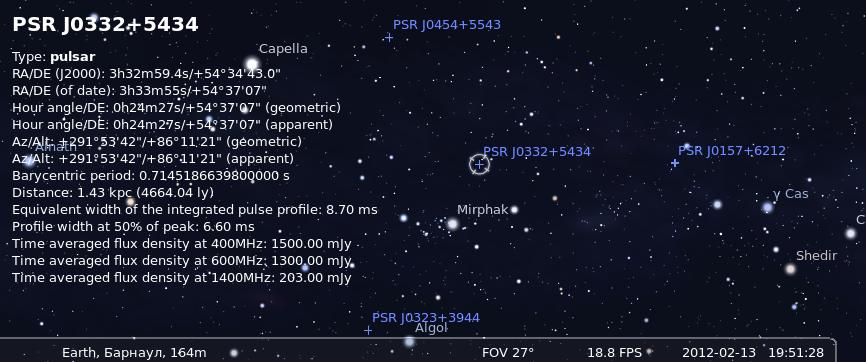
\includegraphics[width=\textwidth]{psr_j0332_5434.jpg}
\caption{PSR J0332-5434}
\label{fig:plugin:Pulsars}
\end{figure}

\noindent This plugin plots the position of various pulsars, with object
information about each one. Pulsar data is derived from \citetp{2005AJ....129.1993M}.

If enabled (see section~\ref{sec:Plugins:EnablingPlugins}), use the
\guibutton{0.6}{btPulsars-off.png} button to activate display of
pulsars. The GUI allows a few configuration options.  You can also
find a pulsar (\key{F3}) by its designation (e.g., \emph{PSR
  J0437-4715}).



\subsection{Section \big[Pulsars\big] in config.ini file}
%\label{sec:plugins:Pulsars:configuration}

\begin{tabularx}{\textwidth}{l|l|X}\toprule
\emph{ID}               & \emph{Type} & \emph{Description}\\\midrule
last\_update                & string & Date and time of last update\\%\midrule
update\_frequency\_days     & int    & Frequency of updates [days]\\%\midrule
updates\_enable             & bool   & Enable updates of pulsars catalog from Internet \\%\midrule
url                         & string & URL of pulsars catalog \\%\midrule
enable\_at\_startup         & bool   & Enable displaying of pulsars at startup of Stellarium \\%\midrule
distribution\_enabled       & bool   & Enable distribution mode for the pulsars \\%\midrule
flag\_show\_pulsars\_button & bool   & Enable displaying pulsars button on toolbar \\%\midrule
marker\_color               & R,G,B  & Color for marker of the pulsars \\%\midrule
glitch\_color               & R,G,B  & Color for marker of the pulsars with glitches \\%\midrule
use\_separate\_colors       & bool   & Use separate colors for different types of the pulsars \\\bottomrule
\end{tabularx}

\newpage
\subsection{Format of pulsars catalog}
\label{sec:plugins:Pulsars:format}

To add a new pulsar, open a new line after line 5 and paste the following, note commas and brackets, they are important:

\begin{configfile}
"Pulsar designation":
{
    "RA": "Right ascension (J2000)",
    "DE": "Declination (J2000)",
    "notes": "type of pulsar",
    "distance": value of distance based on electron density 
                model (kpc),
    "period": value of barycentric period of the pulsar (s),
    "parallax": value of annular parallax (mas),
    "bperiod": value of binary period of pulsar (days),
    "pderivative": value of time derivative of barcycentric 
                   period,
    "dmeasure": value of dispersion measure (pc/(cm*cm*cm)),
    "frequency": value of barycentric rotation frequency (Hz),
    "pfrequency": value of time derivative of barycentric 
                  rotation frequency (1/(s*s))
    "eccentricity": value of eccentricity,                   
    "w50": value of profile width at 50% of peak (ms),
    "s400": value of time averaged flux density at 
            400 MHz (mJy),
    "s600": value of time averaged flux density at 
            600 MHz (mJy),
    "s1400": value of time averaged flux density at 
             1400 MHz (mJy)    
},
\end{configfile}

%\newpage
\noindent For example, the record for \textbf{PSR J0014+4746} looks like:
\begin{configfile}
"PSR J0014+4746":
{
    "distance": 1.82,
    "dmeasure": 30.85,
    "frequency": 0.805997239145,
    "pfrequency": -3.6669E-16,
    "w50": 88.7,
    "s400": 14,
    "s600": 9,
    "s1400": 3,
    "RA": "00h14m17.75s",
    "DE": "47d46m33.4s"
},
\end{configfile}

\newpage
\section{Quasars Plugin}
\label{sec:plugins:Quasars}

\noindent The Quasars plugin provides visualization of some quasars brighter than 16 visual magnitude. 
The catalogue of quasars has been compiled from \citetp{2010A&A...518A..10V}.

\begin{figure}[ht]
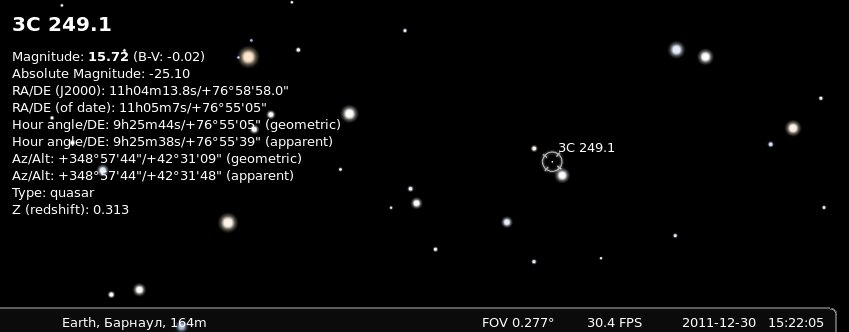
\includegraphics[width=\textwidth]{qso_3c_249_1.jpg}
\caption{3C 249.1, also known as LEDA 2821945 or 4C 77.09}
\label{fig:plugin:Quasars}
\end{figure}


%% TODO follow scheme from Pulsars above. Add a section about QSOs in astornomical phenomena (after galaxies) and add reference from here.


If enabled (see section~\ref{sec:Plugins:EnablingPlugins}), use the
\guibutton{0.6}{btQuasars-off.png} button to activate display of
quasars. The GUI allows a few configuration options.  You can also
find a quasar (\key{F3}) by its designation (e.g., \emph{3C 273}).

\subsection{Section \big[Quasars\big] in config.ini file}
%\label{sec:plugins:Quasars:configuration}

\begin{tabularx}{\textwidth}{l|l|X}\toprule
\emph{ID}               & \emph{Type} & \emph{Description}\\\midrule
last\_update                & string & Date and time of last update\\%\midrule
update\_frequency\_days     & int    & Frequency of updates, in days\\%\midrule
updates\_enable             & bool   & Enable updates of quasars catalog from Internet \\%\midrule
url                         & string & URL of quasars catalog \\%\midrule
enable\_at\_startup         & bool   & Enable displaying of quasars at startup of Stellarium \\%\midrule
distribution\_enabled       & bool   & Enable distribution mode for the quasars \\%\midrule
flag\_show\_quasars\_button & bool   & Enable displaying quasars button on toolbar \\%\midrule
marker\_color               & R,G,B  & Color for marker of the quasars \\\bottomrule
\end{tabularx}

\newpage
\subsection{Format of quasars catalog}
\label{sec:plugins:Quasars:format}

To add a new quasar, open a new line after line 5 and paste the following, note commas and brackets, they are important:

\begin{configfile}
"Quasar designation":
{
    "RA": "Right ascension (J2000)",
    "DE": "Declination (J2000)",
    "Amag": value of absolute magnitude,
    "Vmag": value of visual magnitude,
    "z": value of Z (redshift),
    "bV": value of B-V colour
},
\end{configfile}

%\newpage
\noindent For example, the record for \textbf{3C 249.1} looks like:
\begin{configfile}
"3C 249.1":
{
    "RA": "11h04m13.8s",
    "DE": "+76d58m58s",
    "Amag": -25.1,
    "Vmag": 15.72,
    "z": 0.313,
    "bV": -0.02
},
\end{configfile}


\newpage


\section{Meteor Showers Plugin}
\label{sec:plugins:MeteorShowers}

\begin{figure}[ht]
\includegraphics[width=\textwidth]{meteorshowers.jpg}
\caption{The 1833 Leonids replayed with the Meteor Showers plugin.}
\label{fig:plugins:MeteorShowers}
\end{figure}

\noindent In contrast and extension of the random \emph{shooting stars}
feature of Stellarium (see section~\ref{sec:Phenomena:Meteoroids}), this 
plugin provides data for real meteor showers and a marker for each 
active and inactive radiant, showing real information about its activity. 
If enabled (see section~\ref{sec:Plugins:EnablingPlugins}), just click 
on the Meteor Showers button \guibutton{0.6}{btMS-off.png}  on the bottom
toolbar to display markers for the radiants.


%% TODO: Consider moving to the astronomical phenomena chapter on meteor(oid)s?
\subsection{Terms}
\label{sec:plugins:MeteorShowers:terms}

\paragraph{Meteor shower}
A \indexterm{meteor shower} is a celestial event in which a number of
meteors are observed to radiate, or originate, from one point in the
night sky. These meteors are caused by streams of cosmic debris called
\indexterm{meteoroids} entering Earth's atmosphere at extremely high speeds on
parallel trajectories. Most meteors are smaller than a grain of sand,
so almost all of them disintegrate and never hit the Earth's
surface. Intense or unusual meteor showers are known as meteor
outbursts and meteor storms, which may produce greater than 1,000
meteors an hour.

\paragraph{Radiant}

The \indexterm{radiant} or \indexterm{apparent radiant} of a meteor
shower is the point in the sky from which (to a planetary observer)
meteors appear to originate. The Perseids, for example, are meteors
which appear to come from a point within the constellation of Perseus.

An observer might see such a meteor anywhere in the sky but the
direction of motion, when traced back, will point to the radiant. A
meteor that does not point back to the known radiant for a given
shower is known as a sporadic and is not considered part of that
shower.

Many showers have a radiant point that changes position during the
interval when it appears. For example, the radiant point for the Delta
Aurigids drifts by more than a degree per night.

\paragraph{Zenithal Hourly Rate (ZHR)}

The \indexterm{Zenithal Hourly Rate} (ZHR) of a meteor
shower is the number of meteors a single observer would see in one
hour under a clear, dark sky (limiting apparent magnitude of 6.5) if
the radiant of the shower were at the zenith. The rate that can
effectively be seen is nearly always lower and decreases the closer
the radiant is to the horizon.

\paragraph{Population index}

The \indexterm{population index} indicates the magnitude distribution
of the meteor showers. Values below 2.5 correspond to
distributions where bright meteors are more frequent than average,
while values above 3.0 mean that the share of faint meteors is larger
than usual.

\subsection{Section \big[MeteorShowers\big] in config.ini file}
%\label{sec:plugins:MeteorShowers:configuration}

You can edit \file{config.ini} file by yourself for changes of the
settings for the Meteor Showers plugin~-- just make it carefully!

\noindent%
\begin{tabularx}{\textwidth}{l|l|X}\toprule
\emph{ID}            & \emph{Type} & \emph{Description}\\\midrule
last\_update          & string & Date and time of last update \\%\midrule
update\_frequency\_hours & int & Frequency of updates, in hours \\%\midrule
updates\_enable         & bool & Enable updates of the meteor showers catalog from Internet \\%\midrule
url                   & string & URL of the meteor showers catalog \\%\midrule
flag\_show\_ms\_button  & bool & Enable showing button of the meteor showers on bottom bar \\%\midrule
flag\_show\_radiants    & bool & Enable displaying markers for the radiants of the meteor showers \\%\midrule
flag\_active\_radiants  & bool & Flag for displaying markers for the radiants of the active meteor showers only \\%\midrule
enable\_at\_startup     & bool & Enable displaying meteor showers at starup plugin \\%\midrule
show\_radiants\_labels  & bool & Flag for displaying labels near markers of the radiants of the meteor showers \\%\midrule
font\_size              & int  & Font size for label of markers of the radiants of the meteor showers \\%\midrule
colorARG               & R,G,B & Color for marker of active meteor showers with generic data \\%\midrule
colorARR               & R,G,B & Color for marker of active meteor showers with real data \\%\midrule
colorIR                & R,G,B & Color for marker of inactive meteor showers \\\bottomrule
\end{tabularx}


\subsection{Format of Meteor Showers catalog}
\label{sec:plugins:MeteorShowers:format}

To add a new meteor shower, you just need to:
\begin{enumerate}
\item Copy the code of some valid meteor shower;
\item Paste it in the line 6 (right after the ``showers'': \{) of the showers.json document;
\item Replace the information according with your needs.
\end{enumerate}
Note commas and brackets, they are very important! For example, below is a record for \textit{Northern Taurids}:

\begin{configfile}[\footnotesize]
"NTA":
	{
		"designation": "Northern Taurids",
		"activity":
		[
		{
			"year": "generic",
			"zhr": 5,
			"start": "09.25",
			"finish": "11.25",
			"peak": "11.12"
		},
		{
			"year": "2014",
			"start": "10.20",
			"finish": "12.10"
		},
		{
			"year": "2013",
			"start": "10.20",
			"finish": "12.10"
		},
		{
			"year": "2012",
			"start": "10.20",
			"finish": "12.10"
		},
		{
			"year": "2011",
			"start": "10.20",
			"finish": "12.10"
		}
		],
		"speed": 29,
		"radiantAlpha": "58",
		"radiantDelta": "+22",
		"driftAlpha": "5",
		"driftDelta": "1",
		"colors":
		[
		{
			"color": "yellow",
			"intensity": 80
		},
		{
			"color": "white",
			"intensity": 20
		}
		],
		"parentObj": "Comet C/1917 F1 (Mellish)",
		"pidx": 2.3
	},
\end{configfile}

\subsection{Further Information}
\label{sec:plugins:MeteorShowers:Further}

You can get more info about meteor showers here:
\begin{itemize}
\item Wikipedia about Meteor showers: \url{https://en.wikipedia.org/wiki/Meteor_Showers}
\item International Meteor Organization: \url{https://www.imo.net/}
\end{itemize}

\subsection*{Acknowledgements}
This plugin was created as project of ESA Summer of Code in Space 2013\footnote{\url{http://sophia.estec.esa.int/socis2013/?q=about}}.


\newpage

\section{Navigational Stars Plugin}
\label{sec:plugins:NavigationalStars}

\begin{figure}[ht]
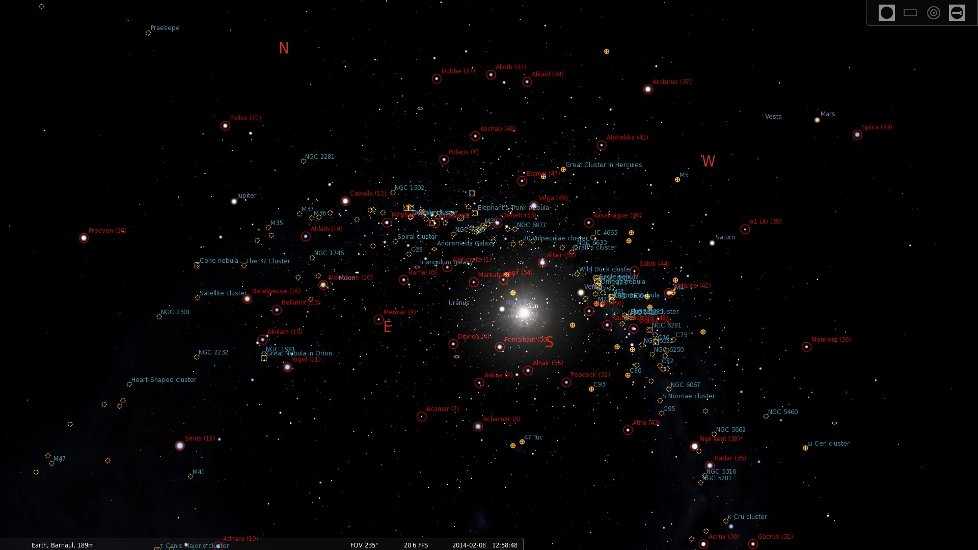
\includegraphics[width=\textwidth]{navstars.jpg}
\caption{Navigational stars on the screen}
\label{fig:plugin:NavigationalStars}
\end{figure}

\noindent This plugin marks navigational stars from a selected set:
\begin{description}
	\item[Anglo-American] --- the 57 ``selected stars'' that are listed in \emph{The Nautical Almanac}\footnote{The Nautical Almanac
		website -- \url{http://aa.usno.navy.mil/publications/docs/na.php}} jointly published by Her Majesty's Nautical Almanac Office and the US Naval Observatory since 1958; consequently, these stars are also used in navigational aids such as the \emph{2102-D Star Finder}\footnote{Rude Starfinder 2102-D
		description and usage instruction --
		\url{http://oceannavigation.blogspot.ru/2008/12/rude-starfinder-2102-d.html}} and \emph{Identifier}. 
	\item[French] --- the 81 stars that are listed in the \emph{Ephémérides Nautiques} published by the French Bureau des Longitudes.
	\item[Russian] --- the 160 stars that are listed in the Russian Nautical Almanac.
\end{description}
If enabled (see section~\ref{sec:Plugins:EnablingPlugins}), just click
on the Sextant button \guibutton{0.6}{bt_NavStars-off.png} on
the bottom toolbar to display markers for the navigational stars. This
can help you in training your skills in astronomical navigation before
you cruise the ocean in the traditional way, with your sextant and
chronometer.


\subsection{Section \big[NavigationalStars\big] in config.ini file}
%\label{sec:plugins:NavigationalStars:configuration}

You can edit \file{config.ini} file by yourself for changes of the
settings for the Navigational Stars plugin -- just make it carefully!

\noindent%
\begin{tabularx}{\textwidth}{l|l|X}\toprule
\emph{ID}			& \emph{Type} 	& \emph{Description}\\\midrule
navstars\_color 	& R,G,B 		& Color of markers of navigational stars  \\
enable\_at\_startup & bool 		    & Set to \emph{true} to display navigational stars at startup of planetarium  \\
current\_ns\_set	& string		& Current set of navigational stars. Possible values: \emph{AngloAmerican}, \emph{French} and \emph{Russian}. \\
\bottomrule
\end{tabularx}


\newpage
\section{OnlineQueries Plugin}
\label{sec:plugins:OnlineQueries}

Stellarium includes and provides lots of information about many kinds
of objects. However, there are scientific websites which provide even
more specialized information about particular objects. This plugin
\newFeature{V0.21.1} allows online access to several websites on a
variety of special topics. To retrieve information, select the
respective tab and press \button{Query}.

\begin{description}
\item[Wikipedia] The free online encyclopedia provides information
  about many bright stars, the planets, moons and many asteroids, as
  well as many deep-sky objects. The lookup is based on the English
  proper name and opens a new tab in your webbrowser.
\item[AAVSO] The \indexterm{International Variable Star
  Index}\footnote{\url{https://www.aavso.org/vsx/}} of the
  \indexterm{American Association of Variable Star Observers} (AAVSO)
  provides data about variable stars in a new browser tab.
\item[GCVS] The \indexterm{General Catalogue of Variable
  Stars}\footnote{\url{http://www.sai.msu.su/gcvs/}} of the Sternberg
  Astronomical Institute and the Institute of Astronomy of the Russian
  Academy of Sciences in Moscow.
\item[Ancient-Skies] A private project founded in preparation of the
  \indexterm{International Year of Astronomy} 2009 which collects
  information about star names and their mythologies
  \citep{AncientSkies:2011}. The site is preparing a relaunch in 2021.
\end{description}

\noindent For technical reasons, there are two kinds of results: Some
query results are presented in the plugin's dialog, while others with
more complicated output (more external links, \ldots) are presented in
your system's webbrowser.

Regardless of the current program language, the result is always
presented in English or the language of the respective website.

In addition, you can configure up to three further websites. These
must provide some public website which takes a query for a Hipparcos
star number or object name.  For example, the website
\url{https://biblicalastronomy.co/playground/fetch.cfm?Hipp=n}
provides various data and cross-references for a star with Hipparcos
number \texttt{n}.

\subsection{Section \big[OnlineQueries\big] in config.ini file}
%\label{sec:plugins:OnlineQueries:configuration}

You can edit the \file{config.ini} file to change settings of the
OnlineQueries plugin.  The only strings you should need to touch are
the \texttt{customN\_\ldots} entries ($\mathtt{N}\in \left\{ 1, 2,
3\right\}$). The placeholder \texttt{\%1} will be filled by either the
Hipparcos number (if the respective \texttt{customN\_use\_hip} is
\texttt{true}) or by the first English name used in Stellarium. The
other entries decide whether to open the result in a webbrowser (if it
is further structured) or in the GUI panel. The
\texttt{customN\_use\_hip} should be \texttt{true} to use a star's
Hipparcos number, or \texttt{false} to use the English name as key.


\begin{center}
{\scriptsize
\begin{tabular}{l|l|l}\toprule
\emph{ID} & \emph{Type} & \emph{Default}\\\midrule
ancientskies\_url    &string & (don't override)\\ % https://www.ancient-skies.org/api.php?apikey=fZdn9QsNdCAY4KggkV2T\&response=HTML\&entity=star\&catalog=HIPPARCOS\&id=\%1 \\
aavso\_hip\_url      &string & (don't override)\\ % https://www.aavso.org/vsx/index.php?view=api.object\&ident=HIP\%1 \\
aavso\_oid\_url      &string & (don't override)\\ % https://www.aavso.org/vsx/index.php?view=detail.top\&oid=\%1      \\
gcvs\_url            &string & (don't override)\\ % http://www.sai.msu.su/gcvs/cgi-bin/ident.cgi?cat=Hip+\&num=\%1    \\
wikipedia\_url       &string & (don't override)\\ % https://en.wikipedia.org/wiki/\%1 \\
\midrule
custom1\_url         &string & https://biblicalastronomy.co/playground/fetch.cfm?Hipp=\%1 \\
custom2\_url         &string & \\
custom3\_url         &string & \\
custom1\_in\_browser &boolean& false\\
custom2\_in\_browser &boolean& false\\
custom3\_in\_browser &boolean& false\\
custom1\_use\_hip    &boolean& true \\
custom2\_use\_hip    &boolean& true \\
custom3\_use\_hip    &boolean& true \\
\bottomrule
\end{tabular}
}
\end{center}


\newpage
\section{Satellites Plugin}
\label{sec:plugins:Satellites}

%% GZ: Found on Wiki on 2016-04 with a deprecation note. Still better than nothing!
%% Original URL: http://www.stellarium.org/wiki/index.php/Satellites_plugin
%% TODO: Update from there or write new.

\noindent The Satellites plugin displays the positions of artifical satellites in Earth's orbit based on a catalog of orbital data. It allows
automatic updates from online sources and manages a list of update
file URLs.

To calculate satellite positions, the plugin uses an implementation of
the SGP4/SDP4 algorithms (J.L. Canales' \program{gsat} library), using
as its input data in NORAD's two-line element set
(TLE\footnote{TLE: \url{https://en.wikipedia.org/wiki/Two-line_element_set}})
format. Lists with TLEs for hundreds of satellites are available
online and are regularly updated. The plugin downloads the lists
prepared by \url{https://celestrak.com} to keep itself up-to-date, but the users can
specify other sources online or load updates from local files.

If enabled (see
section~\ref{sec:Plugins:EnablingPlugins}), just click on the
Satellite button \guibutton{0.6}{bt_hint.png}  on the bottom
toolbar to display markers for the satellites.

It should now be possible to search for artificial satellites using
the regular search dialog (\key{F3}). Note that at any given time, most
Satellites will be below the horizon.

\begin{figure}[htbp]
\centering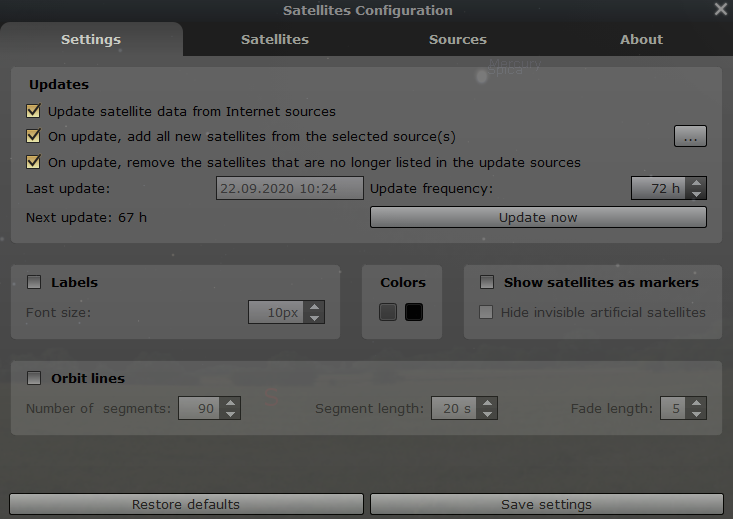
\includegraphics[width=0.8\textwidth]{satellites_plugin_configuration.png}
\caption{Configuration of the Satellites plugin.}
\label{fig:plugins:Satellites:Configuration}
\end{figure}

\subsection{Satellite Properties}
\label{sec:plugins:Satellites:properties}

\begin{description}
\item[Name and identifiers] Each satellite has a name. It's displayed as a label of the satellite hint and in the list of satellites. Names are not unique though, so they are used only
for presentation purposes.

\item[Satellite Catalog] In the \emph{Satellite Catalog} satellites are uniquely identified by their NORAD number, which is encoded in TLEs.

\item[Grouping]
A satellite can belong to one or more groups such as ``amateur'',
``geostationary'' or ``navigation''. They have no other function but
to help the user organize the satellite collection.  Group names are
arbitrary strings defined in the Satellite Catalog for each satellite
and are more similar to the concept of tags than a hierarchical
grouping. A satellite may also not belong to any group at all.

By convention, group names are in lowercase. The GUI translates some of the groups used in the default catalog.
\end{description}

\begin{figure}[tbp]
	\centering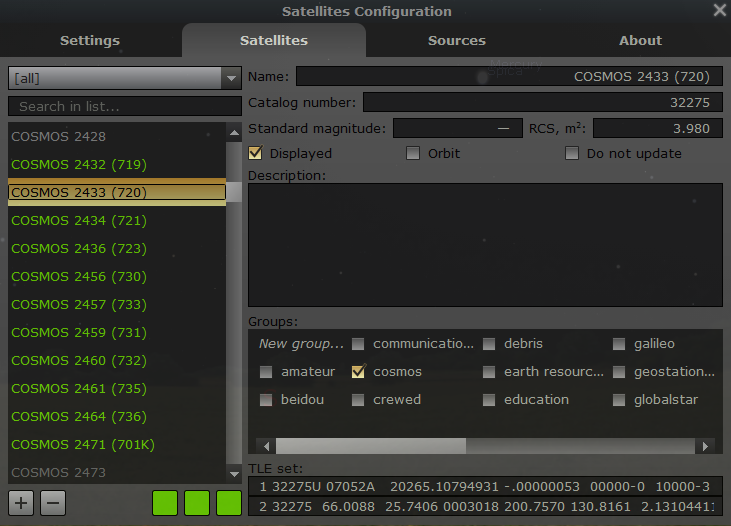
\includegraphics[width=0.8\textwidth]{satellites_plugin_satellites.png}
	\caption{Configuration of the Satellites plugin --- satellites properties.}
	\label{fig:plugins:Satellites:Configuration:Satellites}
\end{figure}


\subsection{Satellite Catalog}
\label{sec:plugins:Satellites:catalog}

The satellite catalog is stored on the disk in JSON\footnote{\url{https://www.json.org/}}
format, in a file named \file{satellites.json}. A default copy is embedded in the plug-in at compile time. A working copy is kept in the user data directory.

%   Used in Satellites plug-in 0.7.1 and later (Stellarium 0.11.2 and later) 

To add a new satellite, open a new line after line 5 and paste the following, note commas and brackets, they are important:
\begin{configfileScr}
"NORAD number": 
{
  "name": "name of the satellite"
  "description": "description goes here",
  "comms": [
     {
  	"description": "downlink 1",
  	"frequency": 437.49,
  	"modulation": "AFSK 1200 bps"
     },
     {
  	"description": "downlink 2",
  	"frequency": 145.825
     }
  ],
  "groups": ["group1", "group2"],
  "stdMag": 2.0,
  "tle1": "1 12345U 90005D   09080.85236265  .00000014  00000-0  20602-4 0  5632",
  "tle2": "2 12345 98.2700  53.2702 0011918  71.1776 289.0705 14.31818920   653",
  "visible": true
},
\end{configfileScr}
Explanation of the fields:

\begin{description}
\item[NORAD number]  required parameter, surrounded by double quotes (\texttt{"}),
followed by a colon (\texttt{:}). It is used internally to identify the
satellite. You should replace the text \texttt{"NORAD number"} with the first number on both lines of the TLE set (in this case, \texttt{"12345"}). It must match the number of the satellite in the source you are adding from if you want the TLE to be automatically updated.
\end{description}
The remaining parameters should be listed between two curly brackets and the closing curly bracket must be followed by a comma to separate it from the next satellite in the list:

\begin{description}
\item[name] required parameter. It will be displayed on the screen and used
when searching for the satellite with the Find window. Use the
description field for a more readable name if you like. (The
description field can accept HTML tags such as \texttt{<br/>} (new line), \texttt{<b></b>} (bold), etc.)

\item[description] optional parameter, double quoted. Appears when you click on the satellite \item[comms] optional parameter, square bracketed list of curly bracketed communications information.
\item[groups]  optional parameter, comma separated list of double quoted group names contained in square brackets. Used for grouping satellites in the drop down box on the config (see above)
\item[tle1]  required, line 1 of the TLE, must be contained in double quotes and begin with \texttt{"1~"}
\item[tle2]  required, line 2 of the TLE, must be contained in double quotes and begin with \texttt{"2~"}
\item[visible]  required parameter, set to true if you want to see it, this can be toggled from the configuration window once the satellite is loaded. 
\item[stdMag]  optional parameter, contained standard magnitude of satellite. 
\end{description}
You can edit the tags for a satellite, modify the description and comms data, and even add new satellites. 

\subsection{Configuration}
%\label{sec:plugins:Satellites:configuration}

The plug-in's configuration data is stored in Stellarium's main configuration
file.

\subsection{Sources for TLE data}

\begin{figure}[tbp]
	\centering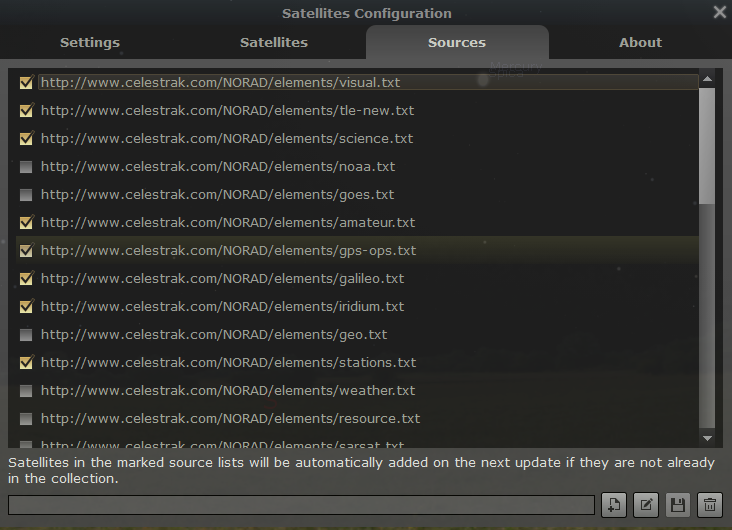
\includegraphics[width=0.8\textwidth]{satellites_plugin_sources.png}
	\caption{Configuration of the Satellites plugin --- sources for TLE data.}
	\label{fig:plugins:Satellites:Configuration:Sources}
\end{figure}

\begin{description}
\item[Celestrak]\footnote{\url{https://celestrak.com/NORAD/elements/}} used as default update source, it also has TLE lists
  beyond those included by default in Satellite plug-in
\item[TLE.info]\footnote{\url{https://www.tle.info/joomla/index.php}}
\item[Space Track]\footnote{\url{https://www.space-track.org/}} the definitive source, requires sign-up, operated by
  United States Department of Defense
\end{description}

%\subsection{Iridium Flares prediction?}
%\label{sec:plugins:Satellites:IridiumFlares}
%
%Some satellites can cause ``flares'' when reflective surfaces divert sunlight towards the observer.
%
%In earlier versions the Satellite plugin could predict ``Iridium flares'' for the current
%location up to 2 weeks in the future from the current moment.
%
%The generation of satellites with highly reflective antennae which
%caused predictable flares has been de-orbited by end of 2019 and
%replaced by models with different geometry which do not cause these
%bright spectacles. \newFeature{v0.20.2} A few defunct satellites are still in orbit, but
%their orientations and flare events are no longer predictable, therefore the
%``Iridium flares'' dialog has been removed.

%%% Local Variables: 
%%% mode: latex
%%% TeX-master: "guide"
%%% End: 

